%\change{Todos los capítulos deben empezar con un p\'arrafo de este estilo. Usar verbos en presente en tercera (ej. realiza, describe, etc.).}
%\change{Colocar la primera letra en may\'uscula cuando se usa el comando ref. Por ejemplo Figura XX, Cap\'itulo XX, Secci\'on XX, Tabla XX. - HECHO}%solucionado en todos los capitulos
%\change{Como el siguiente p\'arrafo:\\
%cifrar en vez
%de encriptar\\
%" o “ cambiarlas por ``(apertura) y '' (cierre)}%solucionado
%\change{algunas figuras est\'an muy grandes, rediseñarlas para optimizar el espacio. Que sean m\'as anchas que largas, para que se aproveche el ancho de la p\'agina}
%\change{Todos los títulos de secciones y cap\'itulos debe ir la primera letra de cada palabra en mayúsculas salvo art\'iculos y preposiciones-HECHO}%solucionado en todos los capitulos
%\change{Graficas con titulo en new roman}


%MAL
%\st{En este cap\'itulo  se profundiza en lo que concierne a este estudio, el ransomware, uno de los tipos de malware con m\'as impacto en la actualidad, su evolución hist\'orica, las diferencias con respecto otros tipos de malware, las familias más importantes, las t\'ecnicas de prevenci\'on y una secci\'on una sección que explica c\'omo lidiar con un equipo infectado por ransomware. Pero para contextualizar, primero se considera necesario exponer conceptos fundamentales sobre el malware, sus tipos y su modelo de negocio.  }

\noindent En este capítulo se realiza un estudio detallado sobre ransomware. Los conceptos fundamentales sobre el malware, sus tipos y su modelo de negocio se presentan en la Sección \ref{sec:2-1}. Los tipos de malware con mayor impacto en la actualidad. En la Sección \ref{sec:2-2} se define el ransomware y se enumeran las principales diferencias con respecto otros tipos de malware. Su evolución histórica, los tipos  y las familias más importantes se detallan en la Secciones \ref{sec:2-3} a \ref{sec:2-5}. En la Sección \ref{sec:2-6} se exponen los diferentes vectores de ataque y los métodos de operación analizan en la Sección \ref{sec:2-7}.  Las técnicas de detección y prevención de los ataques de ransomware así como las recomendaciones para el post-ataque se explican en las Secciones \ref{sec:2-8} a \ref{sec:2-10}.

\section{Malware}\label{sec:2-1}
\noindent Malware es una abreviación de software malicioso. Se trata de programas o fragmentos de código que ganan acceso o provocan daño en un ordenador, sin necesidad de que su propietario lo sepa. El malware utiliza canales de comunicación populares como el correo electrónico o descargas desde páginas web para expandirse. Su finalidad es explotar vulnerabilidades del sistema. Este software ajeno se instala en el equipo y realiza tareas no deseadas, como la aparición de continua y molesta publicidad en la pantalla, pero incluso puede ser utilizado para obtener beneficios económicos a terceros, mediante el robo de información o infección de redes \cite{mwdef}. El malware se clasifica dependiendo de su modo de operación, que pueden ser los siguientes \cite{virusbomb}:
\begin{enumerate}
    \item \textbf{Auto-replicación}: Intenta propagarse mediante las copias o instancias de él mismo. De modo análogo, otros tipos de malware se copian de manera pasiva, por error de algún usuario, por ejemplo.
    \item \textbf{Expansión de la infección}: Describe la capacidad de crecimiento en el número de instancias creadas. Aquellos que se reproducen mediante auto-replicación crecen de manera mucho más rápida. 
    \item \textbf{Parasitario}: Requiere otro código ejecutable para existir.
\end{enumerate}

\subsection{Tipos de Malware}
\noindent Los tipos de malware más importantes son:

\begin{itemize}
    \item \textbf{Virus}: Un virus es un tipo de malware parasitario y con crecimiento exponencial que, cuando se ejecuta, intenta replicarse en otro código ejecutable. Cuando lo consigue, se dice que dicho código ha sido infectado. El código infectado, cuando se ejecuta, puede a su vez infectar nuevo código. Este modo de auto-replicarse en código existente en un computador es la característica definitoria de un virus. Tradicionalmente, los virus se pueden propagar en un solo ordenador, o migrar de unos a otros, transportados a través de un humano, vía \gls{USB}, \gls{CD-ROM} o \gls{DVD}, pero nunca a través de ninguna red \cite{virusbomb}.
    
    \item \textbf{Spyware}: Una clase de código malicioso que se instala de manera encubierta en la máquina de la víctima, y una vez activo, silenciosamente monitoriza el comportamiento de los usuarios, graba sus hábitos al navegar en la red y sustrae sus archivos sensibles y contraseñas. También permite realizar capturas de pantalla, obtener información de la cámara y el micrófono, evitar ser desinstalado e incluso instalar software \cite{articleSpy}.  Normalmente, la información recogida es enviada al distribuidor de \textit{spyware}, y posteriormente utilizada para realizar estudios de publicidad o marketing, e incluso vendida a terceros. Una de las técnicas más importantes es explotar las vulnerabilidades de los navegadores \cite{Egele2007DynamicSA}.
    
    \item \textbf{Adware}: Es considerada una forma menos dañina de \textit{spyware}. Mientras que el \textit{spyware} trabaja de manera encubierta, el \textit{adware} es evidente. Algunas de sus formas de actuar pueden ser cambiar la página de inicio de un navegador, modificar el contenido de páginas web para insertar anuncios, realizar un seguimiento del comportamiento del usuario y transmitir dicha información, que puede ser manteniendo o no la privacidad del usuario, para obtener algún beneficio \cite{articleSpy}.
    
    \item \textbf{Trojans}: Denominados así en referencia al caballo de madera utilizado por los griegos en el asedio a Troya, debido a que el código malicioso entra en el equipo camuflado, normalmente mediante algún archivo descargado al abrir un correo electrónico extraño. Este tipo de malware parasitario permite a su creador ejecutar comandos sin autorización en un equipo infectado. Permite a los \textit{hackers} modificar ajustes de los archivos, robar información o contraseñas, realizar daños en el equipo, apagarlo o incluso
    deshabilitar antivirus u otros mecanismos de seguridad. Actúan según la Figura \ref{fig:imtroyano} \cite{trojan}.
    
     \begin{figure}[htb!]
        \begin{center}
        \subfigure[Fase I]{
            {\scalebox{.6}{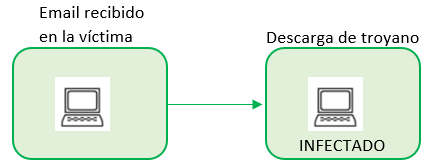
\includegraphics{images/troyano1.png}}}
            \label{fig:troj1}}
        \subfigure[Fase II]{
            {\scalebox{.6}{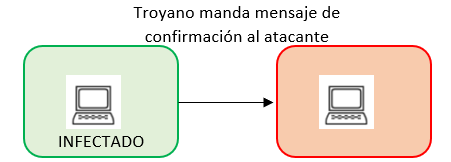
\includegraphics{images/troyano2.png}}}
            \label{fig:troj2}}
        \subfigure[Fase III]{
            {\scalebox{.6}{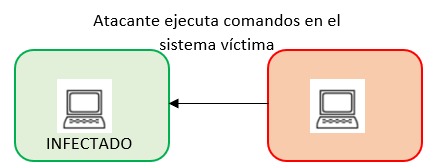
\includegraphics{images/troyano3.png}}}
            \label{fig:troj3}}
        \caption{Flujo de acción de un troyano}
        \label{fig:imtroyano}
        \end{center}
        \end{figure}
    
    
    
    \item \textbf{Worms}: Es un código malicioso que se origina en un único ordenador y busca otros equipos conectados a un área local \gls{LAN} o mediante una conexión a Internet. Cuando el gusano encuentra otro ordenador, se replica en dicho equipo y continúa buscando más ordenadores. Un gusano sigue intentando replicarse indefinidamente o hasta que expira un temporizador, tal como muestra la Figura \ref{fig:im4} \cite{trojan}.
    %\change{Usar la primera letra en mayúscula Figura XX, la Tabla XX. La figura 2.1 no está clara}
    
    \begin{figure}[htb]
    \begin{center}
    {\scalebox{.8}{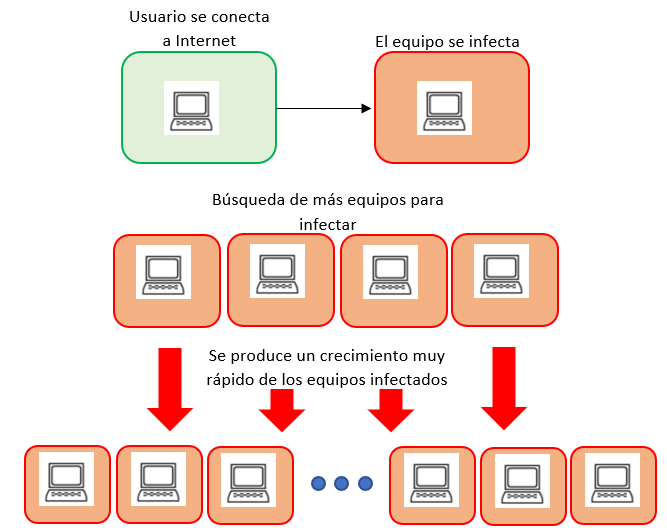
\includegraphics{images/gusano.png}}}
    \end{center}
    \caption{Infección de equipos por gusano}
    \label{fig:im4}
    \end{figure}
    
    \item \textbf{Logic Bomb}. Código malicioso que consiste en una ``carga explosiva'', que puede ser cualquier acción maligna para el equipo víctima, y un disparador: una condición booleana que controla cuando se va a ejecutar la ``carga explosiva'' \cite{virusbomb}.
    %\change{" o “ cambiarlas por ``(apertura) y '' (cierre)}
    
    \begin{algorithm}[htb!]
\renewcommand{\lstlistingname}{Algoritmo}
\begin{lstlisting}[language=config, caption={Ejemplo de bomba lógica sencilla}, captionpos=b, firstnumber=1, linewidth=14.4cm]
    //Codigo legitimo
    if fecha is Viernes 13 then
        apagar_ordenador()
    //Codigo legitimo
    \end{lstlisting}
\label{Alg:imx1}
\end{algorithm}
%\change{utilizar esta forma de hacer los algoritmos o trozos de c\'odigos. Referenciar los algoritmos así como las figuras}

        
\end{itemize}
\subsection{Ingeniería Social Aplicada al Malware}
\noindent La ingeniería social consiste en una serie de técnicas psicológicas y habilidades sociales que permiten persuadir a las personas para obtener de ellas información, ya sea personal o profesional, o para conseguir acceso a su sistema o red. Se basa en una metodología que sigue estas fases \cite{GallegosSegovia2017}:
\begin{enumerate}
    \item \textbf{Recogida de información}: En esta fase se obtiene información sobre la víctima para establecer posibles vectores de ataque.
    \item \textbf{Obtención de confianza}: Las personas tienden a revelar información o secretos con aquellos en quien confían. Debido a esto, el atacante trata de obtener una relación de confianza con la víctima.
    \item \textbf{Fase de aprovechamiento}: La relación de confianza establecida da lugar a la petición de información o la acción requerida. 
    \item \textbf{Fase final}: Los resultados obtenidos en la fase anterior son usados para realizar el ataque planeado previamente.
\end{enumerate}
Los tipos fundamentales de ingeniería social utilizados para realizar ataques malware son los siguientes \cite{GallegosSegovia2017}:
\begin{itemize}
    \item \textbf{Ataques técnicos}: No existe interacción física con la víctima. Se usan herramientas como el correo electrónico o las descargas en la web. Su principal amenaza es que intentan parecer entidades reconocidas y fiables, utilizando logos comerciales, platillas de mensajes, etc.
    \item \textbf{Ataques de ego}: Existe un contacto directo entre el atacante y la víctima.  Los criminales ofrecen ayuda demostrando su inteligencia, de forma que las víctimas caen en un tipo de manipulación transparente, y proporcionan la información con facilidad. 
    \item \textbf{Ataques de simpatía}: Se crea una relación de confianza con la víctima, la cual siente empatía por el atacante. Se basa en el uso de técnicas conversacionales para generar una comunicación espontánea, de manera que la víctima se siente segura y expone sus vulnerabilidades.
    \item \textbf{Ataques de acoso}: Se basan en la intimidación, amenazas y coacción para obtener información.
\end{itemize}

\section{Definición de Ransomware}\label{sec:2-2}
\noindent Ransomware, o secuestro de datos, es un tipo de malware, con características típicas de malware, pero a su vez con sus propias peculiaridades. Se basa en la inyección de procesos en programas destino, que provocan la extracción de datos del usuario y permite la comunicación segura con el servidor de mando y control \gls{CyC}. Su principal objetivo es cifrar los archivos privados del sistema víctima o inutilizar el equipo y forzar al pago por su rescate. El código ransomware es relativamente fácil de encontrar por la web, escribir y modificar. Esta simplicidad del código combinada con su naturaleza lucrativa, ha resultado en la generación explosiva de gran cantidad de variantes \cite{DEFRANSW}. 
El ransomware se diferencia de otros tipos de malware por las siguientes características \cite{ransommasive}:

\begin{itemize}
    \item La finalidad del ransomware es extorsionar dinero a las víctimas, sin dañar el sistema operativo o los datos de manera irreversible, mientras que otros tipos de malware únicamente buscan convertir en inoperante el equipo.
    
    \item No requiere privilegios de administrador para cifrar los archivos.
    
    \item La habilidad tanto de cifrar archivos como de modificar su nombre, hace inconsciente a la víctima de la cantidad de archivos cifrados.
    
    \item Utilizan diferentes métodos para evadir mecanismos de seguridad como \textit{firewalls} o antivirus.
    
    \item Algunos tipos conectan el equipo víctima a \textit{botnets} para otros ciberataques posteriores.
    
    \item Los ataques son independientes de la localización geográfica y del lenguaje del área.
    
\end{itemize}

\section{Historia del Ransomware}\label{sec:2-3}

\noindent El ransomware ha sido una amenaza importante para todo tipo de empresas desde mediados de la década del 2000, pero eso no significa que no haya habido ataques anteriores. Su historia se puede estructurar en dos fases según el tipo de acciones malignas que el malware realiza en el equipo \cite{histRansom}:
\begin{enumerate}
    \item \textbf{Bloqueo de equipo}: En esta etapa se restringía el acceso al sistema operativo, obligando a la víctima a pagar un rescate para poder utilizar su equipo. Este tipo de ataques comenzó a acarrear gran riesgo por parte de los atacantes debido a que los expertos informáticos aprendieron a luchar contra ellos atacando directamente a los pagos electrónicos.
    \item \textbf{Cifrado de información}: Con el nacimiento de las cripto-monedas y habiendo eliminado a los intermediarios en los pagos, como los bancos y al ser imposible su rastreo, surge este tipo de ataque, por el cual se pide un rescate a usuarios y empresas tras cifrar archivos con claves robustas, ofreciéndoles mayor cantidad de beneficios de una manera más segura para los atacantes.
    
\end{enumerate}

El primer ransomware conocido fue el AIDS Trojan, también llamado PC Cyborg Trojan. Fue creado en 1989 por Joseph Popp, un biólogo estadounidense, y distribuido a través de disquetes en una conferencia de la OMS y enviados a través de los servicios postales. Estos disquetes venían en sobres con el remitente ``PC Cybor Corporation'' y decían tener información sobre el SIDA, por lo que fueron enviados a investigadores alrededor del mundo. Se distribuyeron alrededor de 20.000 disquetes en más de 90 países. Usaba criptografía simétrica simple para cifrar nombres de archivos del sistema y hacía que las impresoras conectadas imprimieran una nota de rescate pidiendo al usuario enviar \$189 dólares a un buzón en Panamá para que pudieran recibir el software que desbloquearía su ordenador. Este ransomware causó daños severos al campo científico, haciendo que compañías perdieran todo su trabajo de investigación sobre el tratamiento del SIDA \cite{51}, y fue la base para la evolución del ransomware hacia los ataques más sofisticados que se llevan a cabo hoy en día. %Los primeros desarrolladores de ransomware normalmente escribían su propio código de cifrado, pero hoy en día los atacantes dependen cada vez más del \gls{RaaS}, lo que ha llevado al aumento substancial de los ataques. También se aprovechan de métodos de entrega más sofisticados, como campañas de \textit{spear-phishing}, que es un tipo de \textit{phising} más efectivo por estar dirigido a una organización en específico, siendo una estafa más elaborada \cite{53}.


El siguiente gran paso en la evolución del ransomware fue en 1996, cuando dos investigadores presentaron un artículo en la Conferencia de Seguridad y Privacidad de IEEE llamado \textit{Cryptovirology: extortion-based security threats and countermeasures} \cite{54}. Este documento expuso un programa que usaba cifrado de la clave pública para crear código malicioso que afectara al ordenador infectado y extorsionara a las víctimas para que pagaran una cuantía de dinero por el rescate de su sistema. El documento sugirió los términos \textit{cryptoviral extortion} y \textit{cryptovirology} para nombrar este tipo de ciberataque, que es lo que hoy en día se conoce como ransomware \cite{8}.


Antes del 2005 el ransomware no era muy popular entre los delincuentes y no se produjeron ataques importantes. Sin embargo, esto cambió drásticamente en 2005, cuando los desarrolladores de malware comenzaron a utilizar el cifrado en su código malicioso, creando ransomware de tipo Filecoder. Conocido como el primer ransomware moderno, Trojan Gpcoder o GP Code, fue el más notable ya que utilizaba cifrado \gls{RSA} de 1024 bits, un cifrado fuerte en ese momento, lo que dificultaba la recuperación de los archivos afectados y se propagaba adjunto a correos electrónicos, simulando ser una aplicación de trabajo. Después de GPCoder, surgieron otras familias como Krotten y Cryzip \cite{40}.


En 2007 apareció el primer ransomware de tipo Lockscreen llamado WinLock. Este ransomware se hacía con el control de la pantalla de la víctima y mostraba imágenes inapropiadas junto con un mensaje. Este mensaje informaba al usuario que tenía que pagar un rescate a través de \gls{SMS} para desbloquear su sistema \cite{56}.


En 2009 surgió el primer ataque de un ransomware de tipo Scareware llamado Vundo, y esto supuso el salto a la monetización intensiva de este tipo de crímenes, ayudados por la proliferación de plataformas anónimas de pago en línea. Los delincuentes comprendieron que se podía ganar dinero con el ransomware y este hecho fue el detonante del rápido crecimiento del número de amenazas cada vez más complejas. En 2011, estos tipos de ransomware estaban en auge, detectándose 60.000 nuevos ataques, y en 2012, esa cifra había aumentado hasta los 200.000. Se estimó que, a finales del 2012, el mercado negro de ransomware tenía un valor aproximado de \$5 millones. El ransomware más notable que utilizó tales tácticas para hacerse pasar por agencias de la ley fueron Reveton y Kovter. Reveton cobró los rescates utilizando \textit{bitcoins} y tarjetas anónimas de pago como \textit{MoneyPak} \cite{55}.

%Impulsados por el éxito de Reveton, diferentes variantes de ransomware comenzaron a aparecer entre 2013 y 2015.

CryptoLocker apareció en 2013 y usaba criptografía de clave pública y privada (\gls{AES} y \gls{RSA} de 2048 bits) para cifrar y descifrar los archivos de las víctimas. Fue distribuido por un correo electrónico que simulaba proceder de UPS o FedEx y la versión original de CryptoLocker cifraba alrededor de 67 tipos diferentes de archivos y daba a las víctimas 3 días para pagar. El precio del rescate rondaba entorno a 2 \textit{bitcoins} o 100 dólares. En diciembre de aquel año, se descubrió que 250.000 máquinas fueron infectadas y en torno a 42000 \textit{bitcoins} de rescate habían sido pagados.
Esto provocó un crecimiento explosivo en los pagos de rescate, que alcanzaron más de \$325 millones a finales de 2015 \cite{8}. CryptoLocker fue el primer caso de propagación de ransomware a través páginas web infectadas mediante de la \textit{botnet} llamada Gameover Zeus. No obstante, CryptoLocker también se difundía mediante \textit{spear-phishing} o en correos electrónicos no deseados como un archivo adjunto \cite{55}. La desaparición de CryptoLocker por el cierre de sus servidores \cite{cryptoLock}, condujo a la aparición de varias imitaciones como CryptoWall y TorrentLocker. 

En 2015, CryptoWall superó a CryptoLocker como la versión líder de ransomware, que aprovechaba una vulnerabilidad de Java y se distribuía a través de anuncios maliciosos. En este mismo año aparecieron \gls{RaaS}, un modelo por el que los atacantes distribuían su ransomware mediante la web \gls{TOR}, repartiéndose los beneficios entre los autores y los grupos que realizaban el ataque. CryptoWall fue una de las familias más utilizadas entre abril de 2014 y principios de 2016, habiendo ganado más de \$18 millones \cite{52}. En la Figura \ref{fig:imkap}, realizada con los datos de un estudio de Kaspersky \cite{40}, se puede ver la distribución de todas las variantes de ransomware que surgieron entre los años 2014 y 2015, siendo CryptoWall el más popular después de la caída de CryptoLocker.

\newpage

\begin{figure}[h!]
\begin{center}
{\scalebox{.75}{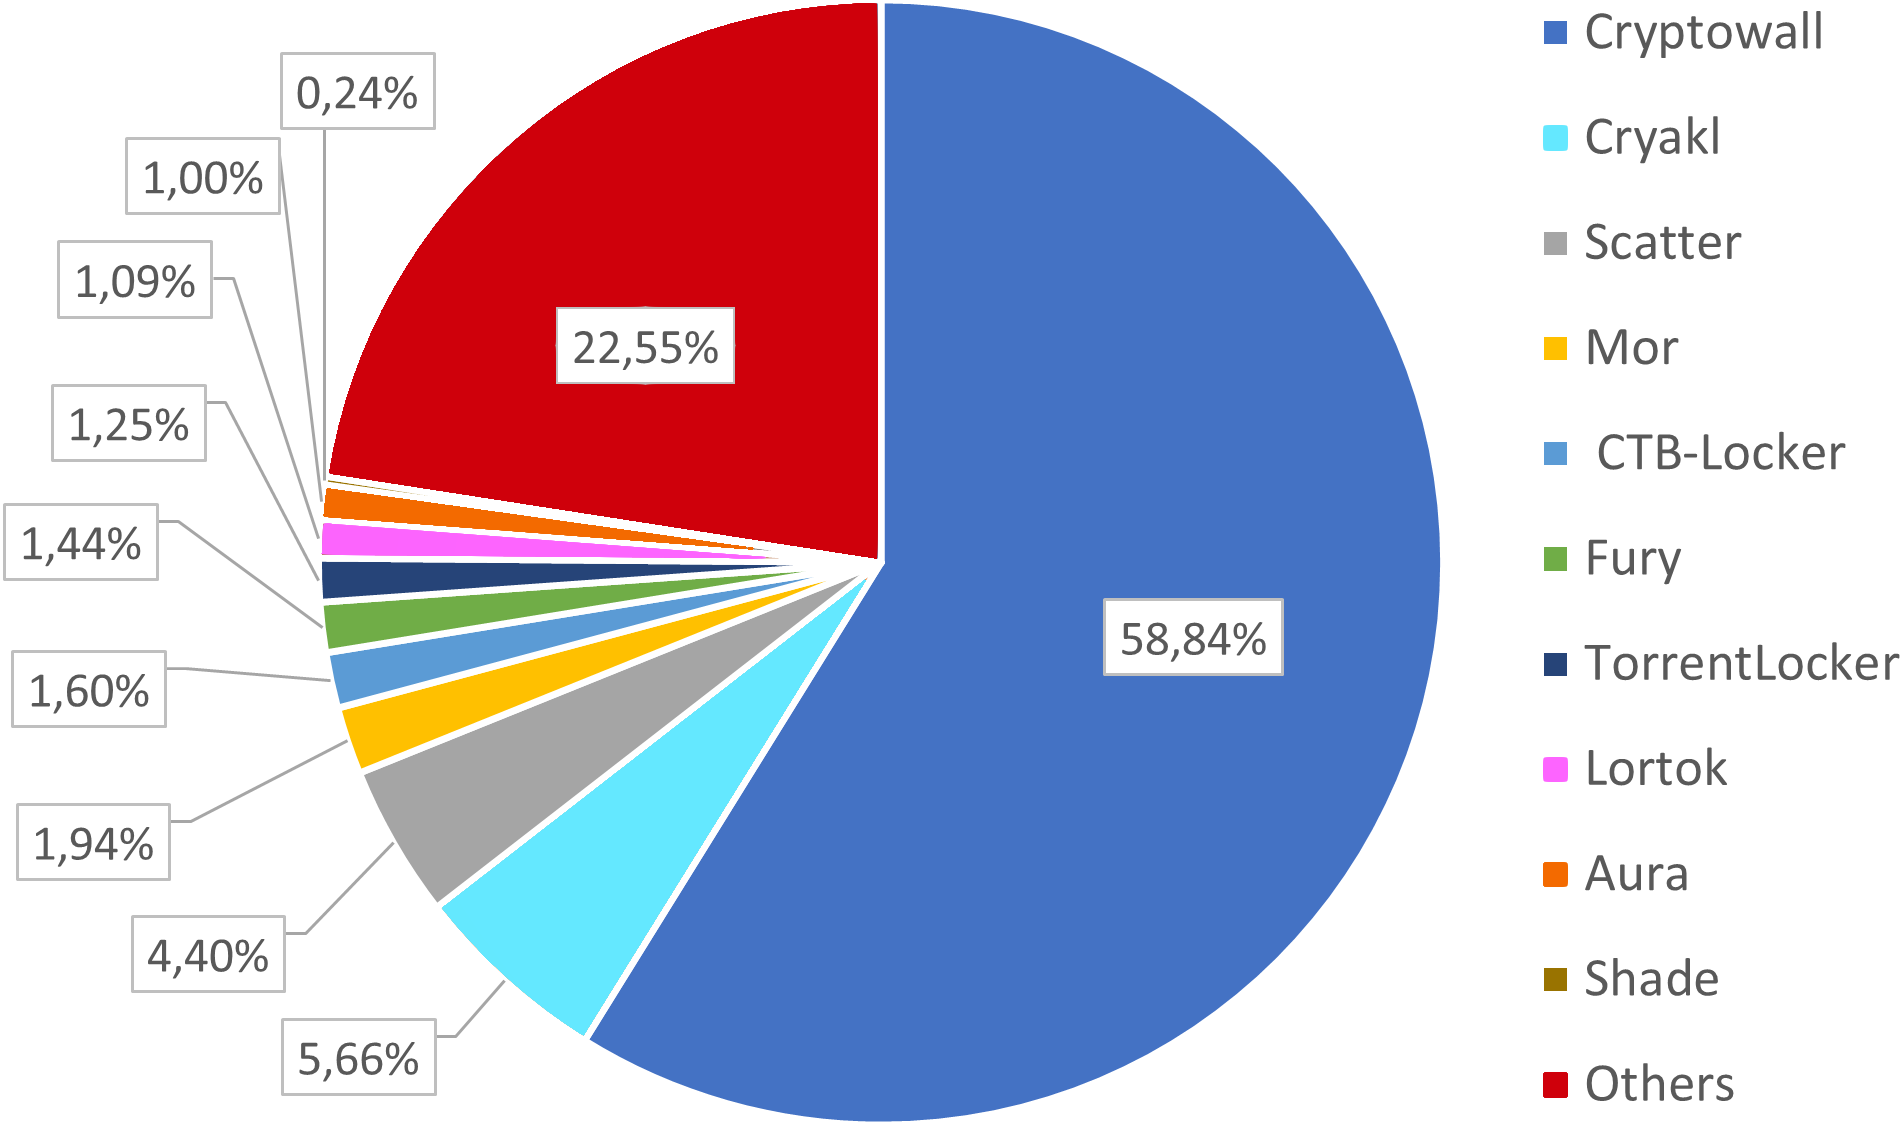
\includegraphics{images/2014-2015.png}}}
\end{center}
\caption{Familias de ransomware más observadas entre 2014 y 2015.}
\label{fig:imkap}
\end{figure}%Marina
%\change{Las gr\'aficas no deben tener el título insertado. Colocar el texto de las figuras en times new roman - HECHO}

En mayo de 2016, ZDNet publicó un artículo \cite{57} donde informaba que las tres principales familias de ransomware más usadas a principios del año fueron Teslacrypt (58,4\%), CTB-Locker (23,5\%) y Cryptowall (3,4\%). A mediados de 2016 surgió Locky y se hizo con el primer puesto, superando a CryptoWall y a Teslacrypt a principios de febrero y solo siendo adelantado por Cerber en junio. El Gráfico \ref{fig:imphish} se ha realizado con los datos de una investigación realizada por PhishMe \cite{6} que estudia todos los hechos mencionados anteriormente.

\begin{figure}[h!]
\begin{center}
{\scalebox{.72}{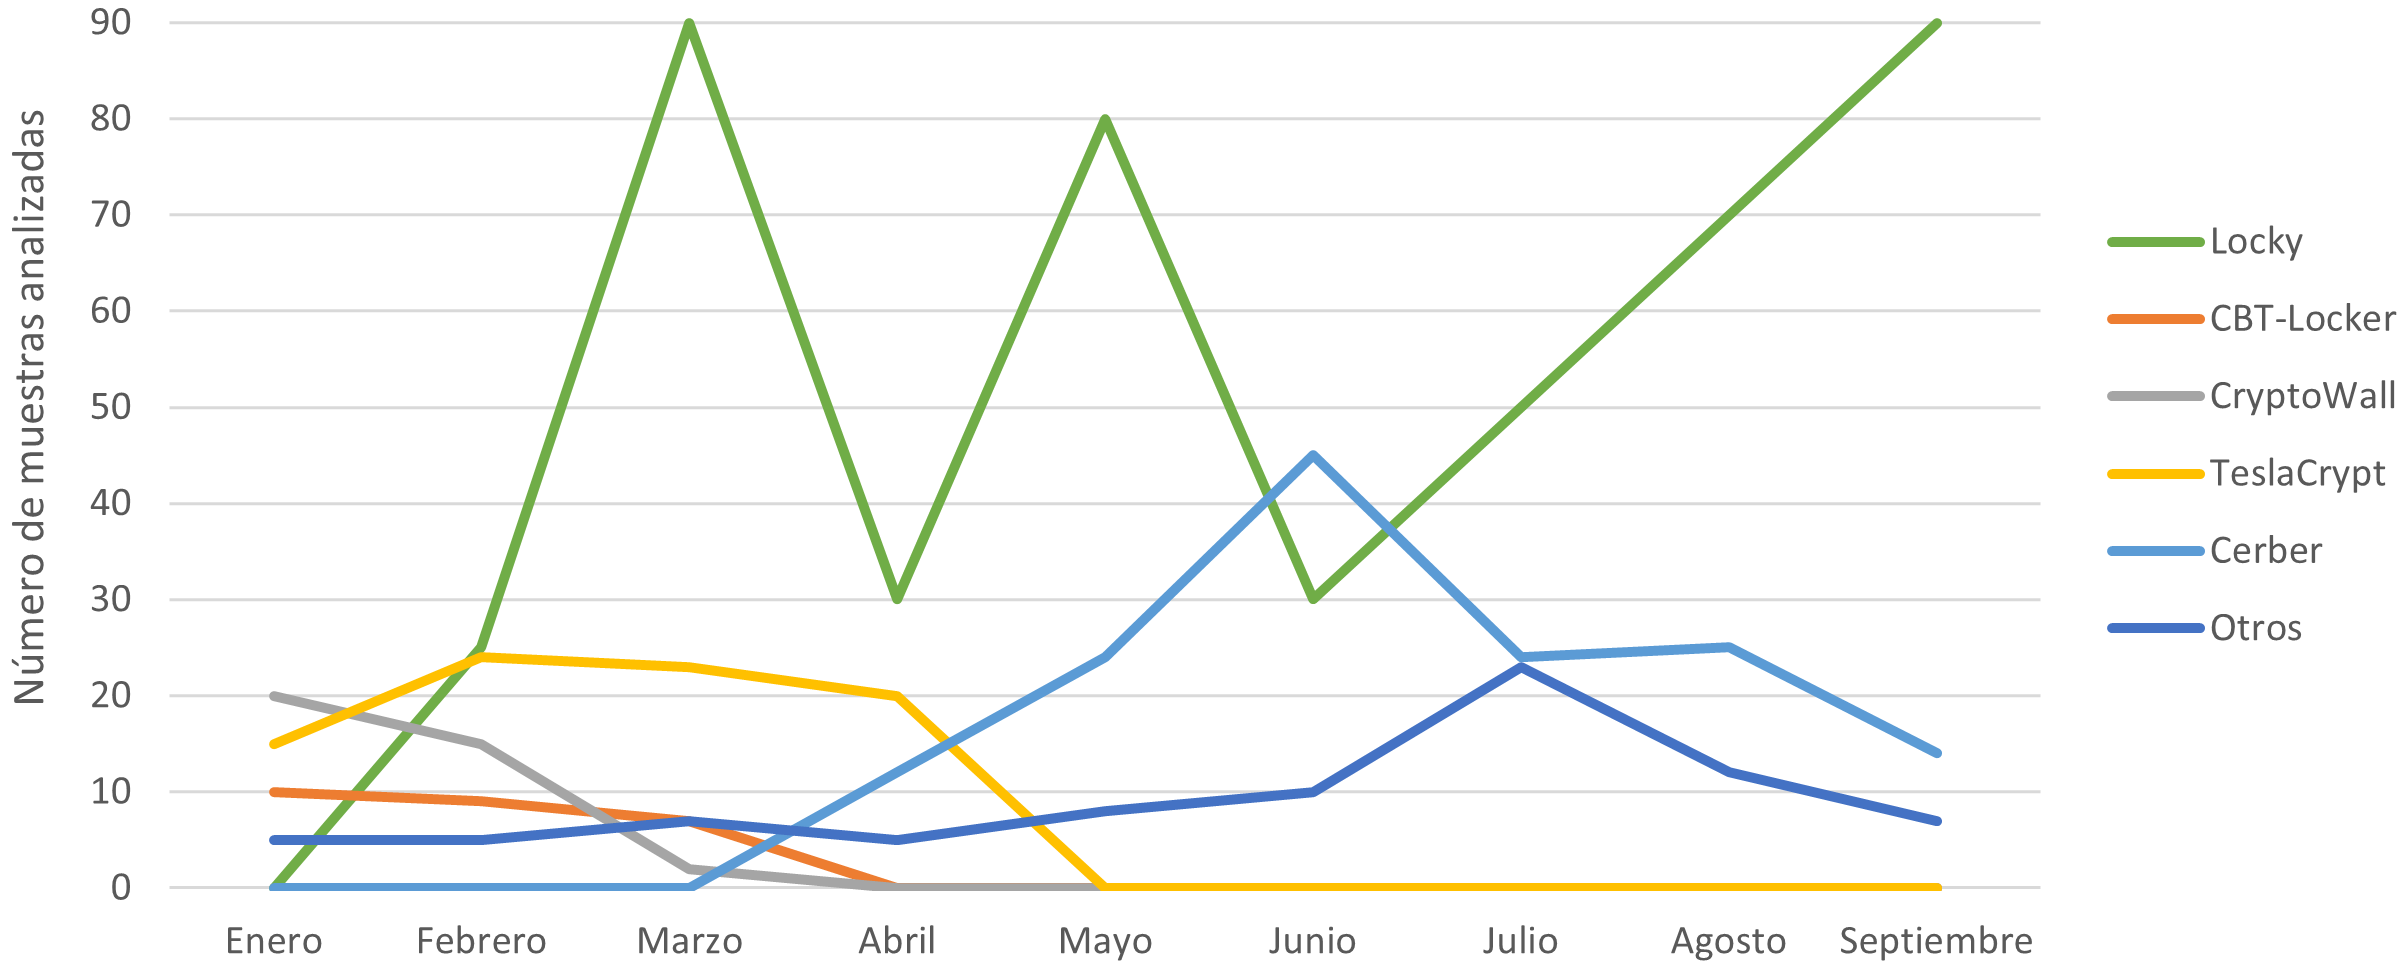
\includegraphics{images/phisme.png}}}
\end{center}
\caption{Familias de ransomware más observadas desde enero hasta septiembre de 2016.}
\label{fig:imphish}
\end{figure}% Marina

%En comparación con las 29 familias de ransomware descubiertas en 2015, en 2016 este número aumentó un 752\%, llegando a 247 en 2016. Los delincuentes recaudaron alrededor de \$1 billón como resultado de atacar a grandes empresas y organizaciones que no tenían copias de seguridad de sus datos, por lo que tuvieron que pagar los rescates \cite{58}. 
%Además, el ransomware continuó su evolución añadiendo nuevas características como contadores para realizar el pago (el rescate se hacía mayor según disminuía) o la propagación por ordenadores mediante la red. Locky, Petya y SamSam fueron las familias más notables descubiertas.

%En 2016 apareció el primer ransomware que atacaba a sistemas Mac \cite{59} y también el primer ransomware llamado ZCryptor que se propagaba automáticamente por los dispositivos conectados a una misma red \cite{60}. Los expertos decían que el 2016 iba a ser un año clave para el ransomware, pero no sabían que lo peor estaba por llegar. 

El año 2017 se consideró por muchos expertos como el ``año de oro del ransomware'', ya que el ataque del ransomware WannaCry fue una epidemia global que sucedió en mayo de ese año. Este ransomware cifraba los archivos de los usuarios, pidiendo \$300 en \textit{bitcoins} por el rescate, y posteriormente esta cifra aumentó hasta los \$600. El 12 de mayo de 2017, WannaCry atacó a sus primeras víctimas en España, en concreto la empresa Telefónica. Días después, el número de usuarios infectados fueron alrededor de 230.000 en más de 150 países, convirtiendo a WannaCry en el mayor ataque de ransomware de la historia. 
Su rápida propagación es debido a que es gusano criptográfico, capaz de replicarse y propagarse automáticamente, aprovechándose de una debilidad en el sistema operativo Microsoft Windows. %siendo capaz de vulnerar cortafuegos y hasta redes privadas virtuales (\gls{VPN}), utilizando herramientas que supuestamente fueron desarrolladas por la Agencia de Seguridad Nacional de los Estados Unidos. 
Este ransomware causó serios daños a bancos, al transporte público, a universidades y a los servicios nacionales de salud, siendo los de Reino Unido los más afectados con costes de alrededor de 92 millones de libras y más de 19.000 citas canceladas \cite{62}.
Además, WannaCry fue el primer ransomware que atacó a los dispositivos \gls{IoT}, en específico a 55 cámaras de tráfico \cite{65}. En definitiva, WannaCry tuvo un impacto importante y se estima que causó pérdidas de alrededor de \$4 billones en todo el mundo \cite{61}.

%Los ataques costaron alrededor del mundo una cifra de 5 billones de dólares, 4 de ellos recaudados por WannaCry, un malware con capacidad para expandirse por las redes, que soporta 27 lenguajes diferentes \cite{ransommasive}.

En 2018 hubo una disminución en los ataques de ransomware. Según los informes publicados por Kaspersky \cite{63} y Malwarebytes \cite{64}, la infección por ransomware cayó un 30\% en todo el mundo, aunque aumentó el número de ataques dirigidos a organizaciones específicas y a dispositivos \gls{IoT}. Estos ataques fueron perpetrados por nuevas variantes de ransomware más sofisticadas, como Ryuk y SamSam. Ryuk atacó a empresas que no se podían permitir periodos de inactividad, como periódicos diarios \cite{66} y una empresa de agua de Carolina del Norte que luchaba contra las secuelas del huracán Florence \cite{67}. %Una característica peligrosa de Ryuk es que puede desactivar la opción restaurar sistema de Windows, lo que dificulta aún más la recuperación de datos cifrados sin pagar un rescate. Las demandas de rescate fueron altas, ya que atacaron empresas con alto valor económico.
SamSam atacó a organizaciones de salud, de educación y de gobierno, explotando el protocolo \gls{RDP} mediante ataques de fuerza bruta y cifrando todos los archivos del sistema. Se estima que el creador de este ransomware ganó alrededor de \$6 millones, ya que atacó a organizaciones tan grandes como el gobierno de Atlanta, que terminó pagando el rescate \cite{9}.

En 2019 se mantuvo la tenencia de lanzar ataques contra organizaciones con gran poder económico y Ryuk siguió siendo un ransomware muy popular entre los criminales junto con Sodinokibi. Sodinokibi o REvil, una variante de GandCrab, fue responsable del cierre de más de 22 pequeñas ciudades de Texas \cite{68} y del ataque a una compañía de cambio de divisas llamada Travelex en la víspera de año nuevo. %Este ataque supuso el cifrado de toda la red de la empresa y el robo de datos personales, incluyendo números completos de tarjetas de crédito de clientes.
Los delincuentes pidieron \$6 millones por el rescate, pero la empresa no pagó \cite{69}.

La Figura \ref{fig:imavg}, creada con datos sacados de un estudio realizado por Crypsis \cite{70}, muestra la media de los rescates pedidos por los delincuentes en los Estados Unidos. Se aprecia un incremento del 140\% entre los dos años, 2018 y 2019 y esto evidencia la situación de que cada vez el ransomware es más sofisticado y ataca a objetivos más grandes con el objetivo de obtener mayores cantidades de dinero. El aumento de la cuantía de los rescates también es debido a que las compañías pagaban a los criminales, lo que les incentivaba a atacar más. En 2018 el 38\% de las empresas afectadas pagaron la suma exigida y en 2019 el 45\%.
%\change{Las gr\'aficas no deben tener el título insertado. colocar el texto de las figuras en times new roman hay texto} 
\begin{figure}[h!]
\begin{center}
{\scalebox{.7}{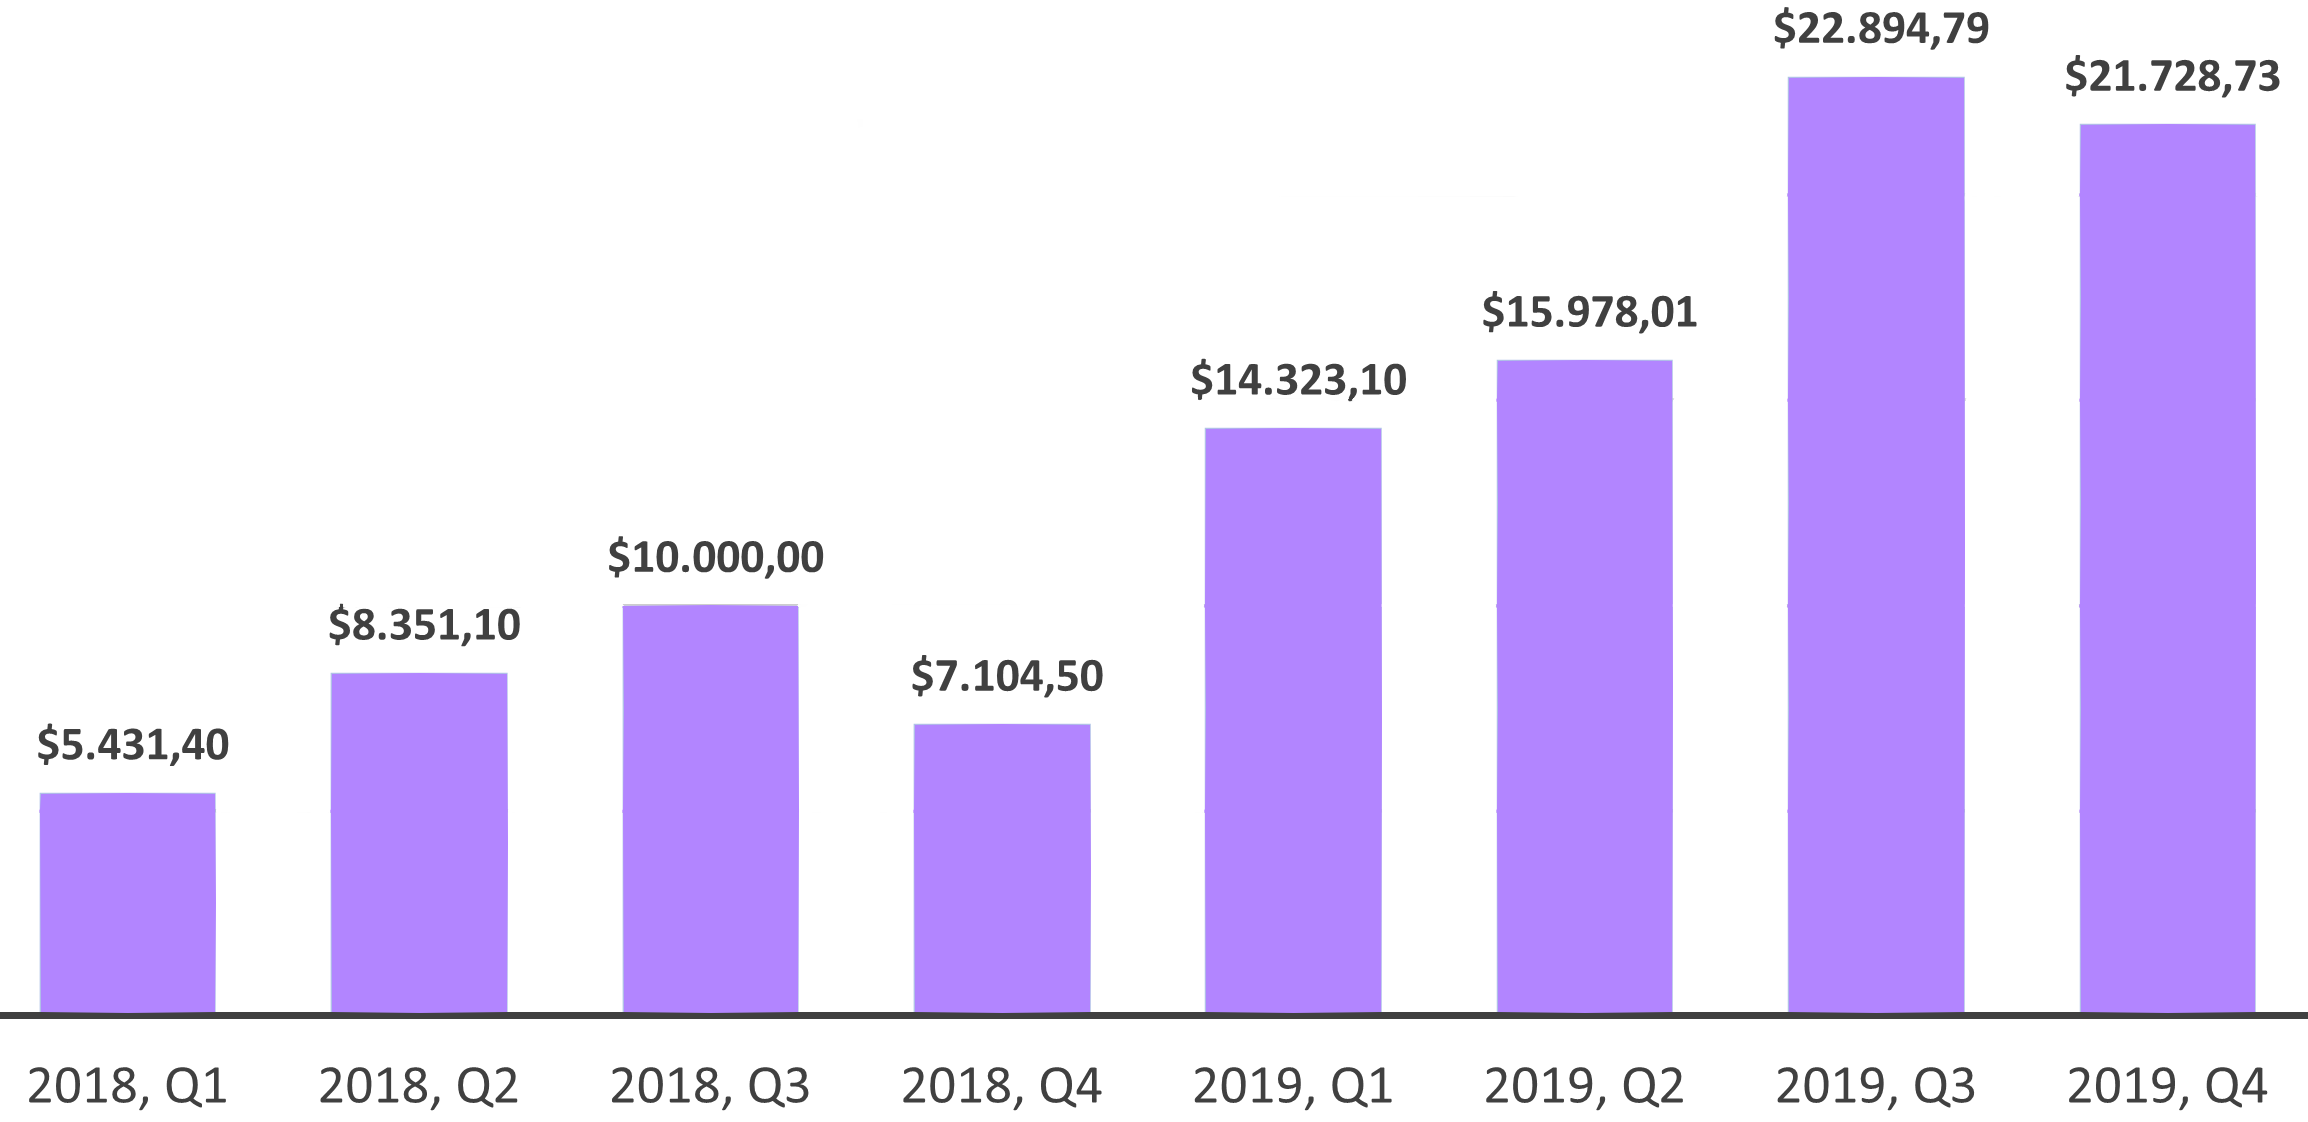
\includegraphics{images/crypsis.png}}}
\end{center}
\caption{Media de la cantidad de dinero que los \textit{hackers} pedían por los rescates en los Estados Unidos (2018-2019).}
\label{fig:imavg}
\end{figure}

En 2020 el ransomware continúa la tendencia de los ataques dirigidos a organizaciones, pero empleando el método de la doble extorsión. No solo cifran y roban los datos, también amenazan con publicarlos si no se pagaba el rescate. Esto supuso una seria amenaza especialmente para las organizaciones más grandes que tienen información altamente confidencial en sus sistemas, y dichos ataques les podrían costar mucho dinero y dañar su reputación e imagen \cite{71}. Maze es un ejemplo de una familia de ransomware que utilizó esta táctica, distribuyéndose de diferentes maneras. La principal fue a través de campañas de \textit{spear-phishing} que instalaban un malware llamado \textit{Cobalt Strike}, pero también infectaba a sistemas con credenciales débiles de \gls{RDP} mediante la explotación de servicios vulnerables de internet para penetrar las redes \cite{25}.
%Gran parte del año 2020 estuvo dominado por las noticias del \gls{COVID-19} y los delincuentes no dudaron en aprovecharse de la crisis y del miedo de las personas. Sucedieron oleadas de campañas de correos electrónicos con archivos maliciosos adjuntos y ransomware dirigido a organizaciones debilitadas o quebradas.
Un estudio realizado por Sophos \cite{38} muestra datos con los que se ha realizado la Figura \ref{fig:imsoph}, que indica el volumen de menciones sobre el \gls{COVID-19} en correos no deseados después de haber sido declarado como pandemia global por la \gls{OMS}.

\begin{figure}[h!]
\begin{center}
{\scalebox{.75}{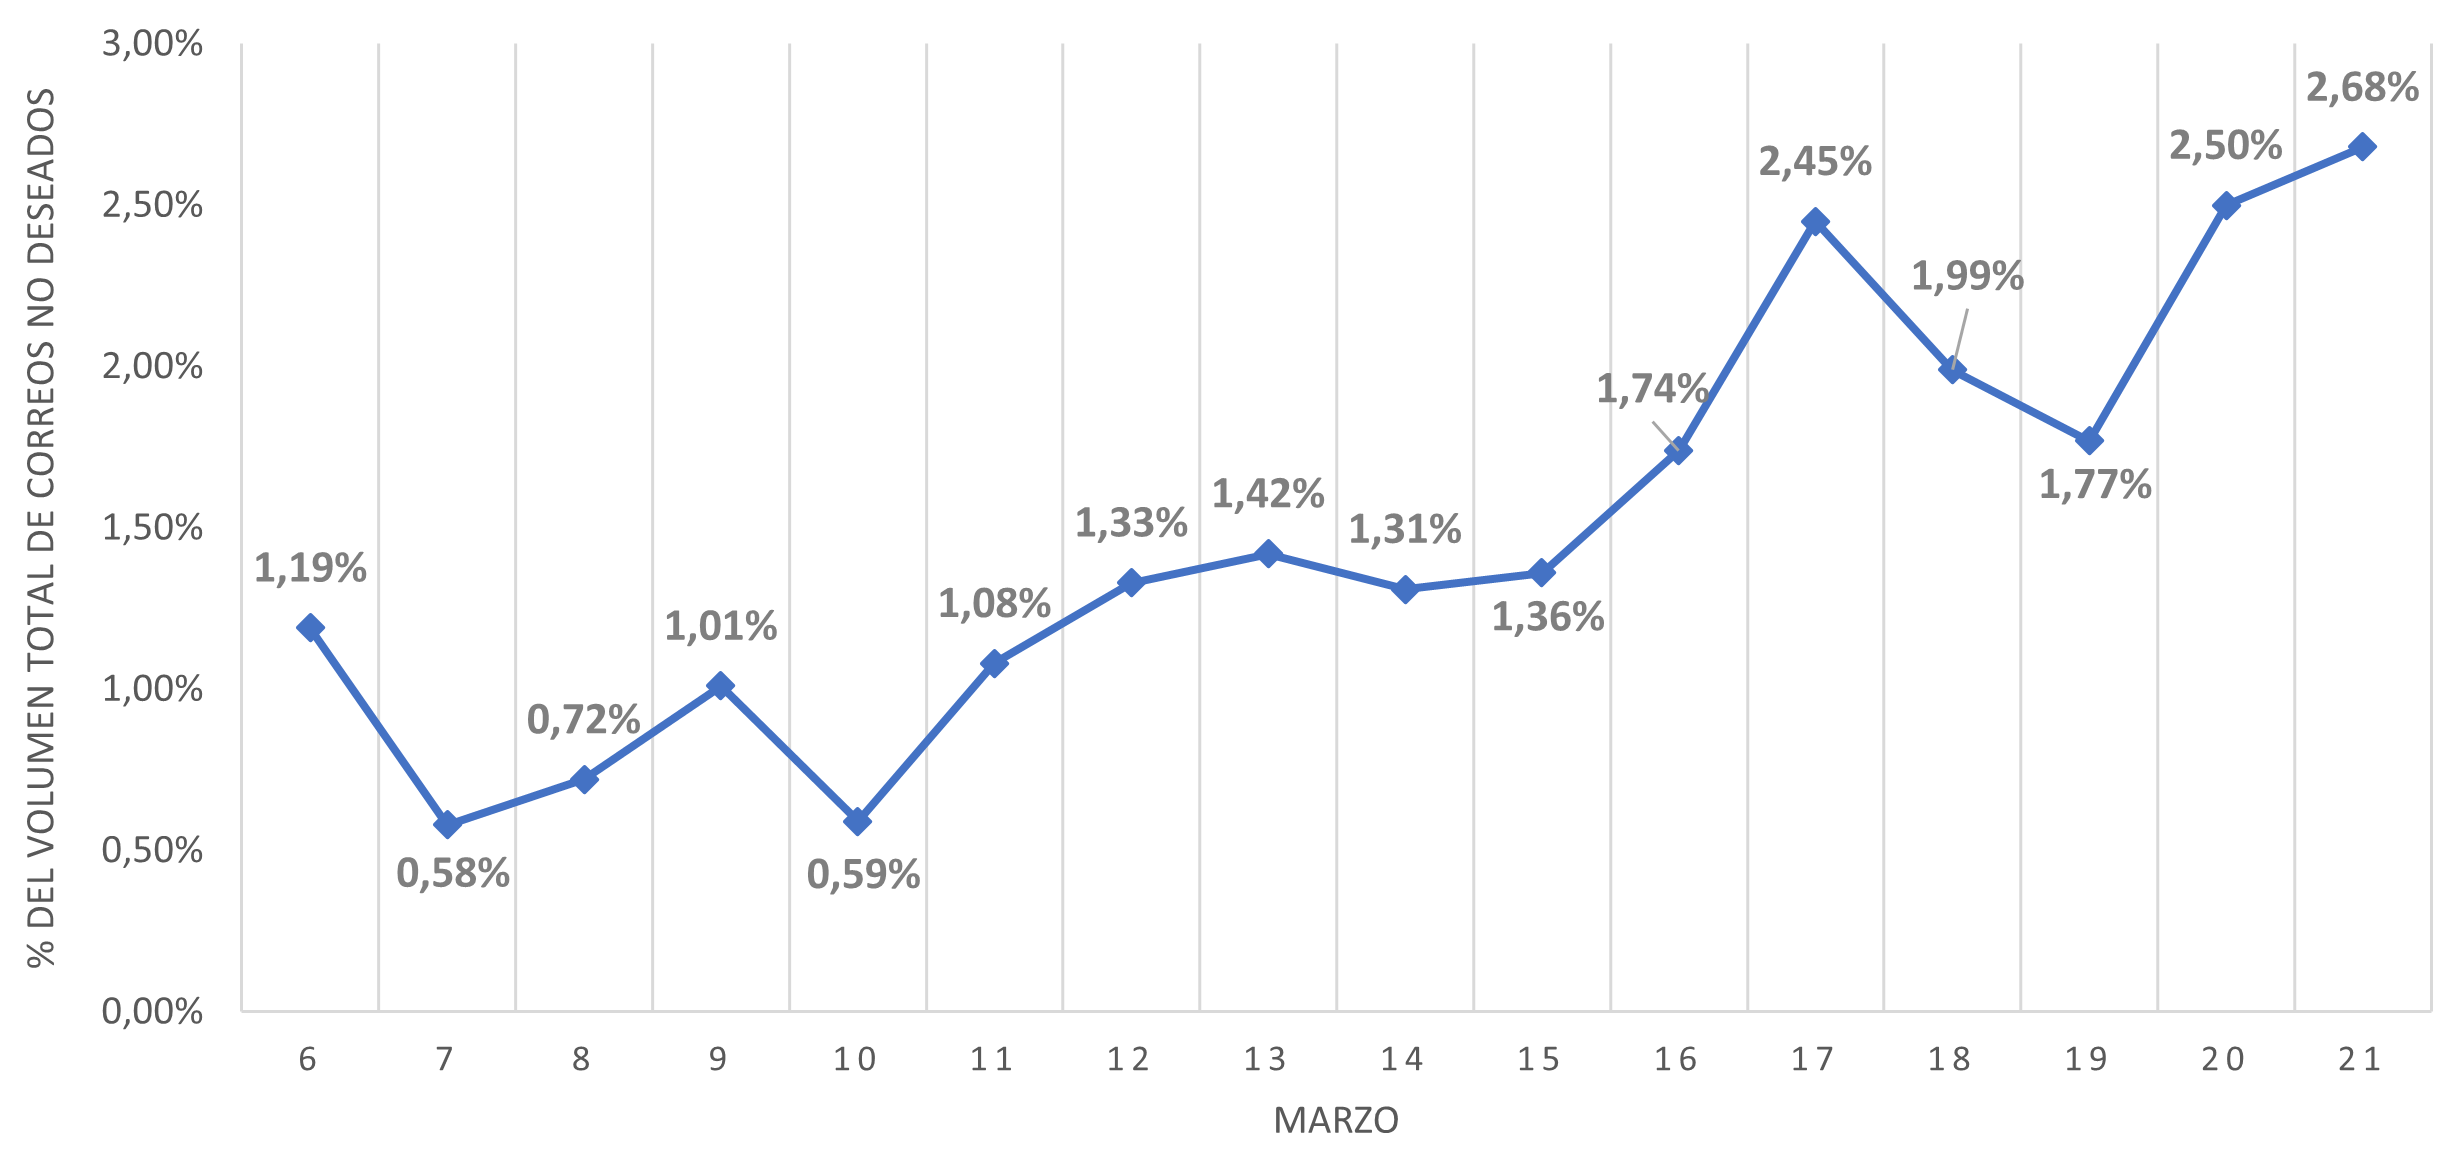
\includegraphics{images/covid_sophos.png}}}
\end{center}
\caption{Volumen de menciones del COVID-19 en correos no deseados de todo el mundo en el mes de Marzo.}
\label{fig:imsoph}
\end{figure}

\begin{comment}

Los expertos pronosticaron un aumento de ataques de ransomware para el 2021 y unas pérdidas mayores para las empresas que están siendo atacadas más y más cada año.
Muchas de las compañías afectadas por ransomware dicen que han experimentado tiempos de inactividad y pérdidas de datos personales, lo que resultó en perdidas millonarias como se puede ver en la Figura \ref{fig:imsafety} creada con los datos sacados de un estudio realizado por SafetyDetectives \cite{72}.

\begin{figure}[h!]
\begin{center}
{\scalebox{.2}{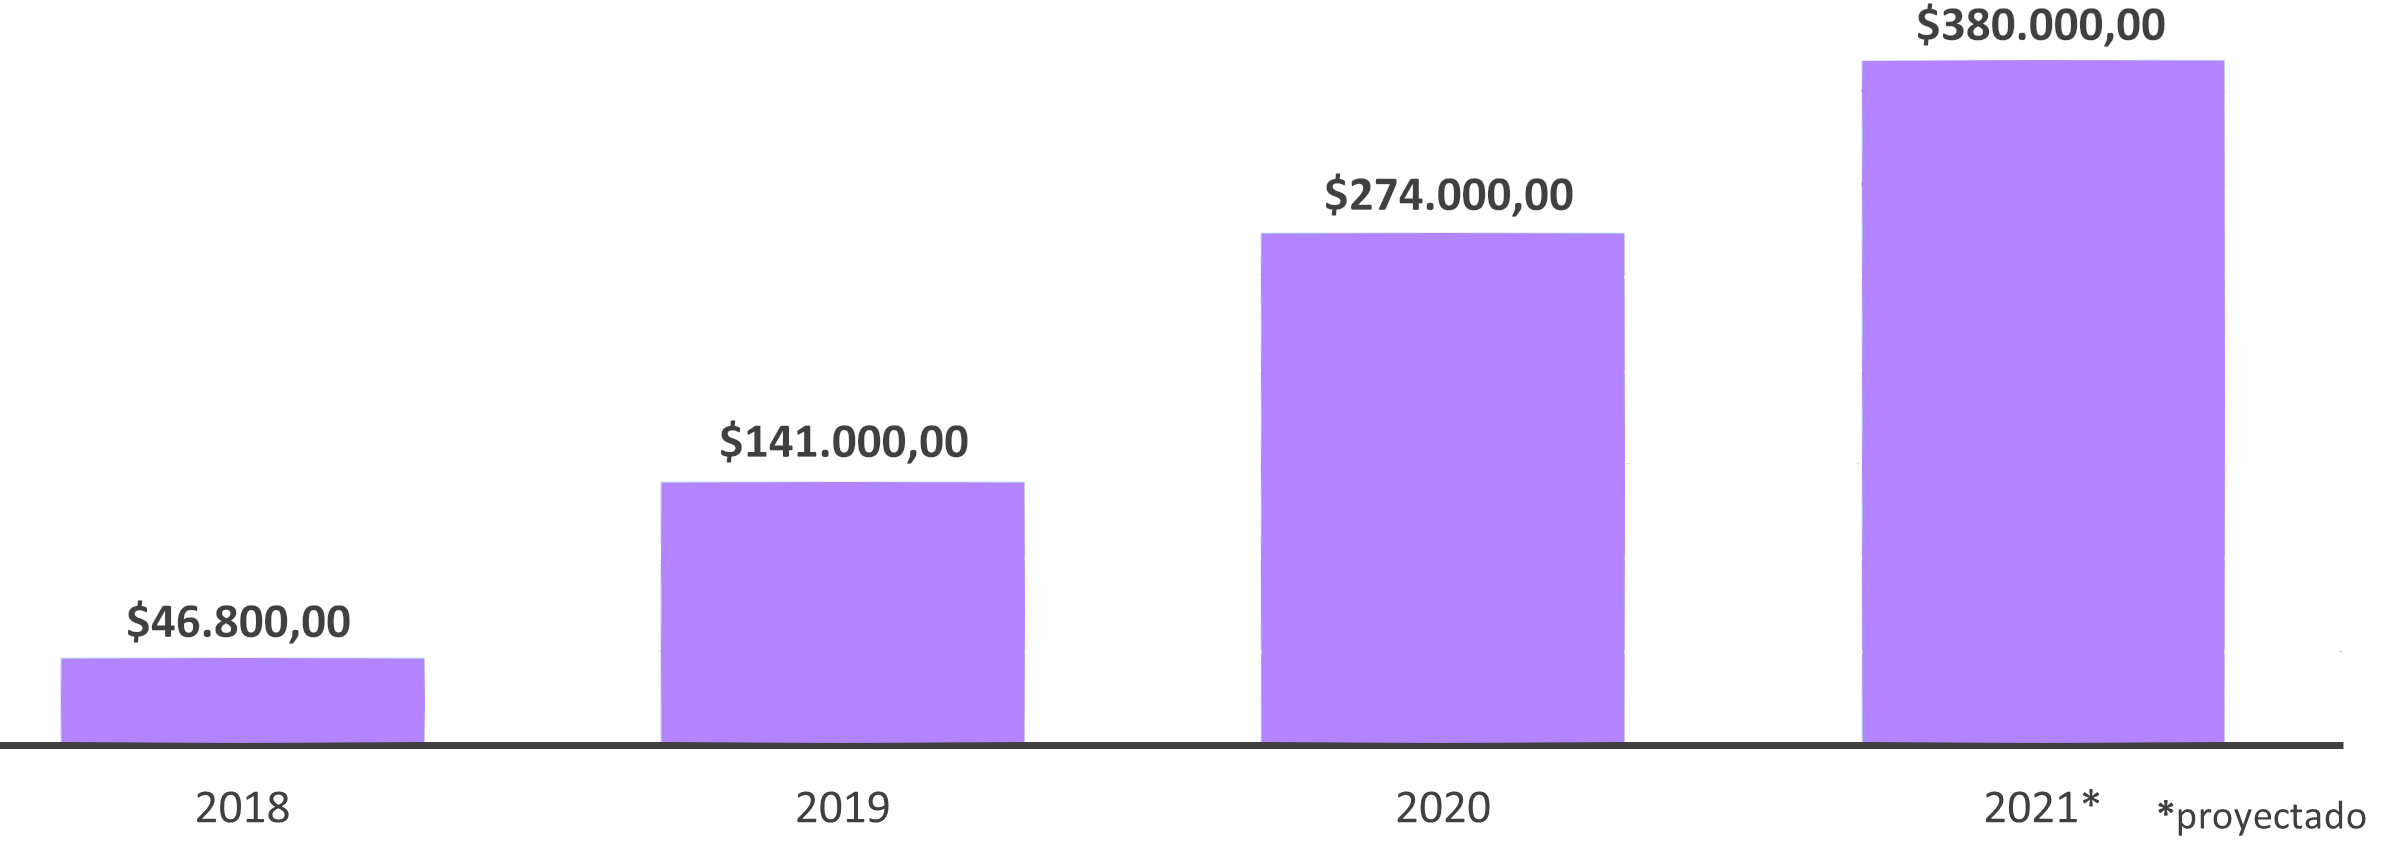
\includegraphics{images/safety_costes.png}}}
\end{center}
\caption{Coste promedio causado por tiempos de inactividad en las empresas afectadas por ransomware.}
\label{fig:imsafety}
\end{figure}


\end{comment}


El primer ransomware del 2021 es Babuk, apareciendo por primera vez en enero y afectando especialmente a empresas de España y Chile. Este ransomware usa su propio esquema de cifrado llamado \textit{ChaCha8}, una variante de Sodinokibi, usando criptografía de curva elíptica. Los precios del rescate oscilan entre \$65.000 y \$85.000 \cite{73}.

En vista de la constante evolución del ransomware, es evidente que las organizaciones son las que están en peligro constante debido a su alto poder económico y a su necesidad de estar operativas todo el tiempo. No se pueden permitir que un ransomware bloquee sus sistemas y tienden a pagar los rescates, sin darse cuenta de que eso solo incentiva a los criminales y no hay certeza de que lleguen a recuperar todos sus archivos y datos afectados. Los criminales pueden intentar negociar y sacar más dinero al ver que la empresa está dispuesta a pagar, por lo que la prevención es clave y la única solución factible. 

La Figura \ref{fig:crono} muestra la cronología de la evolución del ransomware explicada anteriormente, con los ransomware más destacados y los años en los que surgían.
\newpage
\begin{figure}[h!]
\begin{center}
{\scalebox{.4}{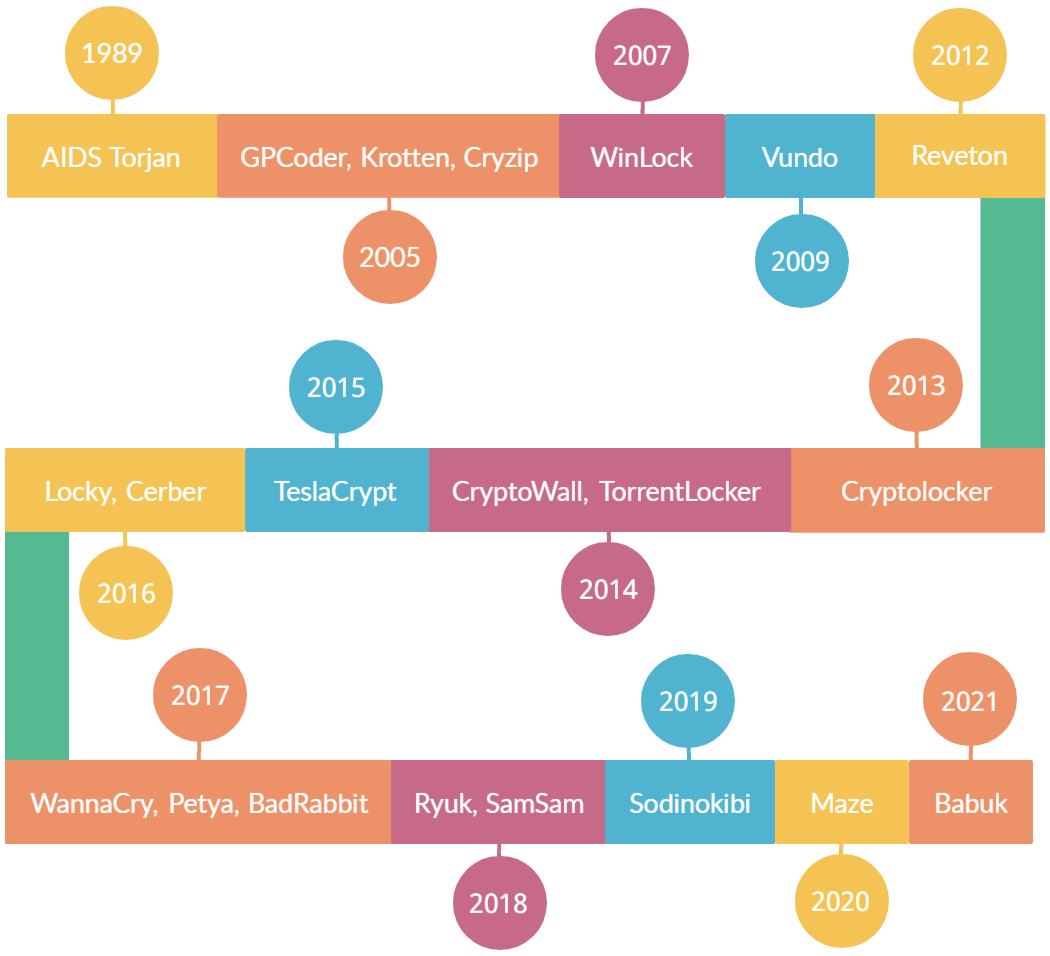
\includegraphics{images/ransomware_timeline.png}}}
\end{center}
\caption{Cronología de la evolución del ransomware.}
\label{fig:crono}
\end{figure}


\section{Tipos de Ransomware}\label{sec:2-4}

\noindent Se identifican dos tipos de ransomware dependiendo de la técnica que utilicen para atacar los sistemas \cite{ransommasive}:

\begin{enumerate}
    \item \textbf{Lockscreen}: Se caracterizan por que bloquean el acceso al sistema a través de la pantalla. En ella se muestra un mensaje indicando que el equipo ha sido infectado y el rescate que deben pagar e imposibilitan al usuario a salir de dicha pantalla.
    Este tipo de ransomware solamente bloquea el acceso a la interfaz del ordenador pero no afecta los archivos. Por lo tanto, existe la posibilidad de eliminar el ransomware y mantener todos los archivos intactos \cite{80}.
    \item \textbf{Filecoder}: Estos ataques cifran archivos del usuario impidiendo el acceso de los usuarios  a su información. Para obtener la clave de descifrado, los usuarios deberán pagar un rescate. Criptolock es el más famoso \cite{79}.
    
\end{enumerate}


En los últimos años además de estos dos tipos han surgido otras variedades que, aunque similares, tienen sus peculiaridades y es importante diferenciarlos para poder comprender su comportamiento y clasificarlos de mejor manera \cite{81}:

\begin{itemize}
\item \textbf{Virus de la policía}: Este ransomware es similar al \textit{Lockscreen}, ya que bloquea el acceso al equipo. La diferencia es el mensaje que muestra al arrancar el sistema, siendo este un mensaje falso de la policía, informando al usuario que se ha detectado accesos a páginas ilegales y que tiene que pagar una multa. 
\item \textbf{Wiper}: Paredico al Filecoder pero más destructivo, ya que bloquea definitivamente el acceso a los archivos y posteriormente los elimina.
\item \textbf{Scareware}: Se hace pasar por un detector de amenazas utilizando ventanas emergentes para informar al usuario sobre supuestos problemas encontrados en su equipo. En lugar de exigir dinero, este ransomware presiona al usuario para que compre un software antivirus falso para resolver todos los problemas instantáneamente. Si el usuario paga e instala el supuesto antivirus, este actuará como malware y recopilará información del equipo y datos personales del usuario \cite{84}.
\item \textbf{Hoax ransomware}: Este ransomware es similar a un Filecoder, pero no cifra ningún archivo ni bloquea el equipo. Simplemente utiliza técnicas de ingeniería social para asustar al usuario y hacerle pagar un rescate falso.
\item \textbf{Leakware}: También llamado \textit{doxware}, este ransomware amenaza al usuario con la publicación de su información personal, como datos confidenciales y conversaciones almacenados si no paga un rescate. Este ransomware es peligroso para las empresas, ya que puede revelar información comprometedora \cite{85}.
\item \textbf{Ataque oculto}: Sucede cuando un usuario simplemente navega a través una página web vulnerada por un \textit{hacker} \cite{82}.
\item \textbf{Dropper}: Infecta al sistema al instalar un programa que en realidad es malware disfrazado, y esto se denomina instalador (\textit{dropper}) de malware. Bad Rabbit, un ransomware que surgió en 2017, se propagó haciendo uso de una solicitud falsa para instalar Adobe Flash, que en realidad era un instalador de malware \cite{83}.
\end{itemize}

Hay otros tipos de ransomware que no tienen un nombre en concreto, pero es conveniente mencionarlas. La reescritura del \gls{MBR} antes de cifrar los datos es una estrategia inusualmente agresiva que usa el ransomware CoViper, y el \gls{FDE} lo realiza el ransomware Mamba. Petya hace algo similar, pero solo cifra la \gls{MFT}, por lo que los datos en si no se ven afectados \cite{82}.


Finalmente, cabe mencionar otras técnicas de extorsionar a las víctimas \cite{ransommasive}:

\begin{enumerate}
    \item \textbf{Scareware}: Este tipo de malware funciona convenciendo a las víctimas para comprar artículos que no necesitan mediante alertas de seguridad falsas.
    
    \item \textbf{Extorsión DDoS}: Puede ser considerado \textit{blackmail} cuando los atacantes solicitan dinero por no realizar un ataque distribuido de denegación de servicio.
    
    \item \textbf{Extorsión por datos comprometidos}: El ciberdelincuente amenaza a la víctima con exponer datos sensibles públicamente a no ser que éste pague un rescate.
\end{enumerate}


\section{Familias de Ransomware}\label{sec:2-5}
\noindent A continuación se listan algunas de las familias más peligrosas y con mas impacto \cite{histRansom} \cite{smartech}:
\begin{itemize}
    
    \item \textbf{Petya}: Tiene dos variantes, una de 2016 y otra, llamada NotPetya, que apareció en 2017. Una vez ejecutado, Petya sobrescribe el sistema de arranque, posteriormente cifra la tabla de ficheros maestros, provocando que Windows sea incapaz de localizar los ficheros almacenados. Posteriormente se reinicia el ordenador, y Petya evita que Windows arranque con normalidad y muestra un mensaje de extorsión como el que se puede observar en la Figura \ref{fig:im5}, procedente del análisis de Cuckoo Sandbox de una muestra realizada en este estudio.
    NotPetya es muy peligroso puesto que puede ser propagada con intervención humana y las claves de cifrado son generadas aleatoriamente y destruidas, lo que hacen que la recuperación de los datos sea imposible \cite{ransommasive}.
    \begin{figure}[htb]
    \begin{center}
    {\scalebox{.5}{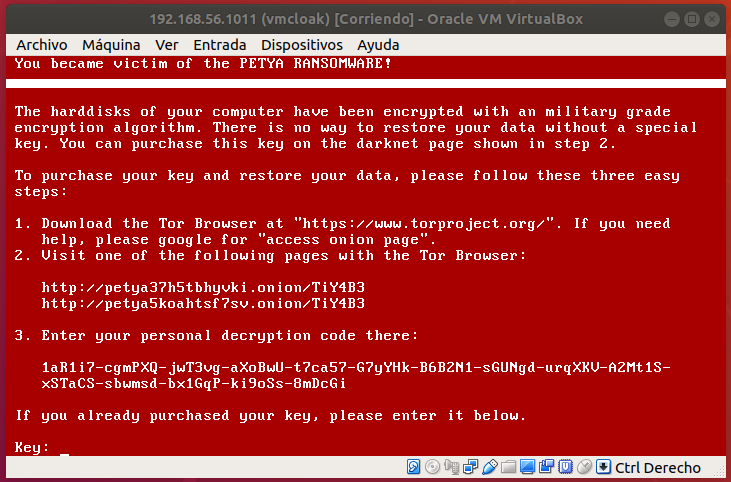
\includegraphics{images/Petya.png}}}
    \end{center}
    \caption{Aviso de extorsión del ransomware Petya}
    \label{fig:im5}
    \end{figure}
    
    \item \textbf{Locky}: Los usuarios se infectan debido a un correo electrónico. Utiliza macros y archivos de \textit{script} para cifrar archivos cuando se abre un documento. Al ejecutarse el \textit{script}, los archivos cifrados se renombran y Locky muestra al usuario una nota de rescate, configurándola como fondo de pantalla. Locky utiliza un algoritmo de cifrado \gls{RSA}-2048+\gls{AES}-128 para cifrar archivos, discos duros e incluso dispositivos extraíbles. Locky ataca a máquinas con base Windows, eliminando el sistema Windows \textit{Shadow Volume Copy} para prevenir cualquier posible recuperación de archivos por parte del usuario.
    
    \item \textbf{SamSam}: Es usado para atacar a una organización, después de haber realizado un estudio y reconocimiento de sus sistemas IT, para reconocer alguna vulnerabilidad en la red o equipos. Afecta a una máquina y se propaga por red a todos las conectadas. Se diferencia a otras familias porque no utiliza técnicas de ingeniería social como correos electrónicos de \textit{spam} o \textit{phising}, sino que los atacantes realizan ataques de fuerza bruta contra las contraseñas débiles para ganar acceso a la red de la organización tras el estudio previamente comentado \cite{ransommasive}. 
    
    \item \textbf{CryptoWall}: Se trata del sucesor de CryptoLocker. Su objetivo son máquinas de base Windows, y se propaga mediante e-mails maliciosos y kits de \textit{exploits} como Nuclear o Angler. Una vez ejecutado en el equipo, escribe su propio registro de auto-arranque, de modo que es resistente a los reinicios. Elimina los sistemas de restauración y procede a cifrar los archivos mediante el algoritmo \gls{RSA}-2048. Su versión más reciente, CryptoWall 4.0 usa un esquema de comunicación con la red \gls{TOR} a través de un servidor \textit{proxy} externo \cite{ransommasive}, como se puede observar en la Figura \ref{fig:imcryp}.
    \begin{figure}[htb]
    \begin{center}
    {\scalebox{.85}{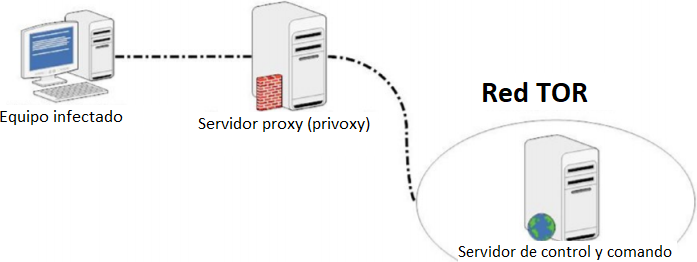
\includegraphics{images/cryptowall.png}}}
    \end{center}
    \caption{Esquema de red de un ataque con Cryptowall}
    \label{fig:imcryp}
    \end{figure}
    
    \item \textbf{CryptXXX}: Familia de ransomware de cifrado que ataca a sistemas operativos Windows. No cifra únicamente los archivos, sino que también ejecuta otro malware de robo de información, como por ejemplo credenciales de VPN, \textit{cookies} o incluso \textit{bitcoins} del ordenador de la víctima y es enviado de nuevo al servidor de control y comando. Utiliza el algoritmo de cifrado \gls{RSA}-4096 y añade la extensión``.crypt'' al nombre del fichero. Posee un sistema anti-sandboxing y anti-analisis \cite{ransommasive}.
    
    \item \textbf{Cerber}: Se diferencia al resto porque es capaz de emitir por los altavoces del dispositivo mensajes de alerta de infección del malware. Incluye ataques a plataformas \textit{Cloud} y \textit{Windows Scripting} y ataques \gls{DDoS}. No solo ataca a máquinas de usuarios individuales, sino que también ha llegado a cifrar bases de datos enteras de empresas.
    
    \item \textbf{Jigsaw}: Debe su nombre a que utiliza como imagen de bloqueo de pantalla al protagonista de la película \textit{Saw}. Infecta archivos de manera exponencial cuanto más tiempo pase sin que la víctima pague el rescate. 
    Posee una característica peculiar que habilita un ``chat'' que ayuda al usuario a pagar para recuperar sus datos.
    
    \item \textbf{CryptoLocker}: Es el primero en utilizar \textit{bitcoin} como moneda de rescate. Accede al sistema utilizando técnicas de ingeniería social, mediante correos electrónicos de empresas de paquetería. Se trata de un ransomware que combina las técnicas de Lockscreen y CriptoLocker.
    
    \item \textbf{WannaCry}: Se diferencia por su éxito de infección, más de 300.000 equipos en más de 150 países fueron afectados por este ransomware debido a una vulnerabilidad de Windows que permite a un atacante remoto ejecutar código arbitrario \cite{exploit}. La dificultad de protegerse contra WannaCry reside en que usa un componente de gusano, que provoca que el ataque sea mucho más efectivo y se necesiten mecanismos de defensa que puedan reaccionar en tiempo real \cite{Akbanov2019}.
 
    \item \textbf{HDDCryptor}: Bloquea la máquina además de afectar a recursos compartidos en la red como impresoras, puertos y archivos a través de \textit{Server Message Block}. Ataca tanto a usuarios individuales como a empresas, y un ejemplo conocido es Mamba.
    
    \item \textbf{Crysis}: También conocido como Dharma, es un ransomware que utiliza ataques de fuerza bruta para propagarse. En 2017, Dharma consiguió que se duplicaran este tipo de ataques por todo el mundo. Esta familia se ha encontrado en 123 países, concentrándose el 60\% de los ataques en 10 países, entre los cuales España ocupa la segunda posición \cite{CcnCert}. 
    
\end{itemize}

En el Anexo \ref{anexo-1} se presenta una lista extendida de las familias de ransomware más conocidas \cite{7}. 

\section{Métodos de Propagación}\label{sec:2-6}
\noindent En esta sección se exponen los diferentes vectores de ataque usados por los creadores de ransomware para invadir los sistemas víctimas \cite{ransommasive}.


\begin{itemize}
    \item \textbf{Ataque de fuerza bruta}: Este ataque sucede cuando los criminales emplean el \gls{RDP} y técnicas para probar una gran variedad de combinaciones de contraseñas, con el objetivo de revelar las credenciales del usuario y así lograr acceso a su sistema \cite{78}.  
    
    \item \textbf{Auto-propagación}: Es la propagación del ransomware de un sistema infectado a otro, difundiendo archivos infectados a todos los contactos disponibles en esa máquina. Antes de iniciar el proceso de cifrado, se expande rápidamente para aumentar sus posibilidades de infectar otros ordenadores \cite{29}.

    \item \textbf{Dispositivos \gls{USB}}: Aunque se trate de un método de propagación primitivo, los cibercriminales siguen utilizándolo para realizar ataques a sistemas. Requiere el acceso físico a algún puerto donde poder conectar el dispositivo ejecutor, aunque existe alguna técnica como esparcir memorias \gls{USB} por diversos lugares con la expectativa de que algún usuario los conecte.
    
    \item \textbf{Drive-by-Downloads}: Los atacantes comprometen sitios web legítimos e incrustan código malicioso en sus páginas, como código \textit{JavaScript}. Este código malicioso realiza publicidad maliciosa, redirecciones engañosas, ataques \gls{XSS} u otros ataques en secreto, sin que el usuario sepa que su sistema está siendo infectado \cite{46} \cite{47}.

    \item \textbf{E-mail}: Es la manera más utilizada, con un 59\%, según un estudio de IBM de 2017 \cite{IBMstats}. Cuando los descuidados usuarios descargan y abren el contenido malicioso, el sistema se infecta de inmediato. También pueden contener \gls{URL} a páginas web maliciosas que infectan el computador. Suelen realizarse mediante campañas de \textit{spam}, e-mails no solicitados enviados a grandes grupos de personas, con el objetivo de realizar promociones. Se trata de algo convincente puesto que, los mensajes de \textit{spam} se contabilizaban como el 53.5\% del tráfico mundial en 2018 \cite{statista}. La técnica más utilizada es el \textit{phising}. Se basa en realizar campañas de \textit{spam} usando el mismo formato que alguna compañía legítima en sus comunicaciones para recaudar información de la víctima. 

    \item \textbf{Botnets troyanos}: El ransomware también puede llegar a un sistema a través de otro malware. Este es el caso de los \textit{Botnets}, que son una red de robots que se ejecutan de manera automática y autónoma. El término \textit{Botnet} surge con una combinación de dos palabras, ``bot'' de robot y ``net'' de red en inglés. Estos robots controlan a los equipos que infectan para que realicen varias tareas, tales como: atacar a otros ordenadores, enviar correos electrónicos no deseados a los contactos del usuario, entregar ransomware, instalar \textit{spyware} y otras actividades maliciosas similares \cite {45}. La Figura \ref{fig:im8} muestra un diagrama de acción de una \textit{Botnet}.

    \begin{figure}[htb]
    \begin{center}
    {\scalebox{.7}{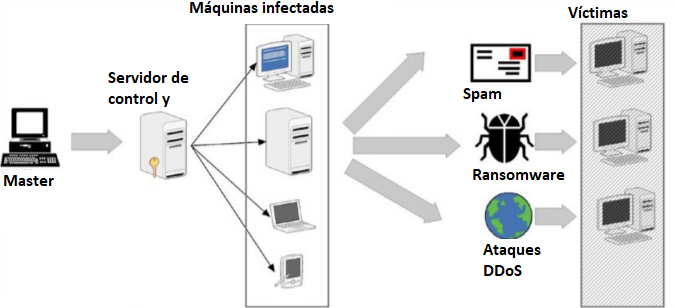
\includegraphics{images/botnet.png}}}
    \end{center}
    \caption{Diagrama de acción de un botnet}
    \label{fig:im8}
    \end{figure}

    \item \textbf{Explotar vulnerabilidades de servidores}: Los criminales explotan las vulnerabilidades del software que se ejecuta en servidores para obtener acceso a la red de una organización y difundir su malware a través de ella \cite{29}.

    \item \textbf{Kits de Exploit}: 
    %Los \textit{exploit kits} aprovechan las vulnerabilidades del software de servidores web para instalar malware, inyectando \textit{iframes} (componentes de un elemento HTML que permiten incrustar contenido) en las páginas web alojadas en ellos. Los \textit{iframes} redirigen a los usuarios que navegan por esos sitios a los \textit{exploit kits}. Se ha visto un aumento del uso de estos kits, especialmente uno llamado \textit{Angler} \cite{30}. Este kit roba las contraseñas del equipo y luego lo infecta con ransomware.
    Se definen como plataformas web que permiten ejecutar \textit{exploits} de manera semi-automática mediante la detección de vulnerabilidades en el sistema operativo o la aplicación víctima y comparándolas con las almacenadas en el kit. Se componen de cuatro partes:
    \begin{enumerate}
        \item \textbf{Página de destino}: Contiene el código responsable para escanear las vulnerabilidades a explotar.
        \item \textbf{Puerta}: fragmento de código que recibe la información de la página de destino y decide si continuar con el ataque o no, según los criterios predefinidos.
        \item \textbf{Exploit}: Explota las vulnerabilidades previamente detectadas ejecutando algún tipo de código malicioso en la máquina víctima para poder acceder a ella.
        \item \textbf{Carga}: Tras haber accedido mediante las vulnerabilidades, el kit de \textit{exploit} envía la carga, algún tipo de malware o algún mecanismo que lo descargue, para realizar el daño real.
    \end{enumerate}
    
    \item \textbf{Malvertising}: Anuncios maliciosos distribuidos a través de páginas web confiables por atacantes que compran espacios publicitarios. Los usuarios que acceden a esas páginas ni siquiera tiene que hacer clic en el anuncio en algunos casos, ya que simplemente cargar la página web que aloja la publicidad maliciosa provocará una infección \cite{44}. Esto era muy común cuando los sitios web usaban Adobe Flash para reproducir anuncios animados \cite{43}.

%La publicidad maliciosa es un tipo de ataque por el que se abusa de canales de publicidad legítimos para propagar malware mediante la inyección de código dentro de los anuncios y las plataformas web. En la práctica, los anuncios maliciosos pueden aparecer como una ventana emergente para llamar la atención del usuario. Si éste hace click en dicho anuncio, se descarga automáticamente el malware.
    
    \item \textbf{Macros de Microsoft Office}\label{item:macros}: Son una serie de instrucciones y comandos para automatizar tares en programas de Microsoft Office como Word o Excel. Los cibercriminales distribuyen por la red ficheros de estos programas con macros maliciosas en ellos y, cuando el usuario las abre, la macro ejecuta funciones malignas para la máquina víctima. 

    \item \textbf{Phishing y técnicas de ingeniería social}: El \textit{phishing} es un ciberataque que usa correos electrónicos como arma, siendo el método más efectivo para distribuir ransomware \cite{41}. Su objetivo es recopilar información personal del usuario mediante correos electrónicos o sitios web maliciosos, engañándole para que acceda a un enlace o que descargue un archivo adjunto. Lo que distingue al \textit{phishing} es la forma del mensaje: los atacantes se disfrazan como una entidad confiable, a menudo una empresa o persona real con la que la víctima podría hacer negocios \cite{42}. Otra técnica de ingeniería social usada comúnmente por los delincuentes es engañar al usuario para que descargue un antivirus falso, y al escanear el equipo con este programa, será infectado por el ransomware.

    \item \textbf{Ransomware as a Service}: \gls{RaaS} es un servicio de ventas de paquetes software de ransomware establecido en mercados negros o foros usando un modelo de suscripción. Se trata de una plataforma emergente muy dañina que permite adquirir software malicioso de manera sencilla. Intervienen tres actores: el autor del código, un proveedor de servicios y los agentes que los adquieren, los futuros atacantes.
    
\end{itemize}

\section{Modo de Operación}\label{sec:2-7}
\noindent Los ataques ransomware siguen las siguientes fases desde que se instalan en el equipo víctima hasta que el usuario puede advertir su presencia \cite{ransommasive}:

\begin{enumerate}
    \item \textbf{Infección}: El ransomware es introducido en el sistema mediante las técnicas detalladas en la Sección \ref{sec:2-6}.
    
    \item \textbf{Ejecución}: Si la infección fue satisfactoria, el ransomware se instala en el equipo víctima y se conecta con el \gls{CyC} mediante el protocolo criptográfico \gls{TLS} y le empezará a enviar información de la víctima de forma segura \cite{35}.
    
    \item \textbf{Destrucción del respaldo}: El ransomware realiza una búsqueda de los ficheros de respaldo y los elimina, de manera que el usuario sea incapaz de recuperar sus archivos. En paralelo, el ransomware también elimina las copias de seguridad del sistema y dependiendo del tipo, también podrá eliminar las \textit{shadow volume copies} (instantáneas) del sistema o cambiar los nombres de los archivos, agregando una extensión relacionada con el nombre de la familia del ransomware \cite{29}. 
    
    \item \textbf{Cifrado}: Se establece una conexión segura con el servidor \gls{CyC} para que le proporcione al ransomware una clave simétrica generada aleatoriamente y este empezará a cifrar los archivos del usuario, usando el algoritmo de cifrado asimétrico \gls{RSA}. Este algoritmo usa dos claves diferentes, una pública para el cifrado de los datos y otra privada para el descifrado  \cite{36}. También pueden usar el algoritmo \gls{AES}, siendo \gls{AES}-256 la forma más común \cite{34}.
    
    \item \textbf{Rescate}: El ransomware reproduce un mensaje de extorsión en la pantalla del ordenador de la víctima, estableciendo un coste y un período de tiempo. 
\end{enumerate}

Los atacantes pueden intentar minimizar la detección del ransomware mediante el uso de certificados digitales legítimos, comprados o robados, para intentar convencer a los software antivirus de que el código es fiable y no necesita ser analizado \cite{39}. Aún así, este método podría fallar, ya que este certificado puede ser revocado en cualquier momento por las autoridades pertinentes, por lo que el ransomware debe actuar rápidamente. Para conseguir rapidez y efectividad, el ransomware dispone de un mecanismo que le ayuda a diferenciar qué archivos son los más importantes para robarlos y cifrarlos primero. La importancia de estos archivos se mide viendo lo relevantes que son para el usuario, comparando cuando se accedieron por última vez y cuando se crearon \cite{33}, dónde están ubicados (el directorio ``Documentos'' suele contener archivos importantes) y su entropía \cite{32}. Si la entropía es demasiado alta o baja, es porque el archivo contiene información aleatoria o simplemente relleno, por lo que el ransomware interpretará que el archivo fue generado automáticamente por el sistema y lo descartará \cite{30}. Otro método más comúnmente utilizado para evitar ser detectado es el aumento de los privilegios mediante el uso de \textit{exploits}, permitiendo a los atacantes instalar programas como \gls{RATS} (herramientas de administración en remoto) para cambiar o borrar datos, crear nuevas cuentas con todos los derechos de usuario y lo más importante, desactivar el software de seguridad \cite{39}.

Todo lo explicado anteriormente es teniendo en cuenta que el ransomware es de tipo Filecoder. Si es de tipo Lockscreen, sigue el mismo patrón excepto por el cifrado de los datos. Después de haber obtenido los privilegios de administrador y de haber enviado la información robada al servidor \gls{CyC}, bloquea el sistema y muestra una alerta al usuario con los pasos a seguir para recuperar el acceso \cite{35}. 

En la Figura \ref{fig:imstages} se representa el patrón de ataque de un ransomware explicado anteriormente, desde que infecta al equipo hasta que demanda un pago por el rescate. 

\begin{figure}[h!]
\begin{center}
{\scalebox{0.23}{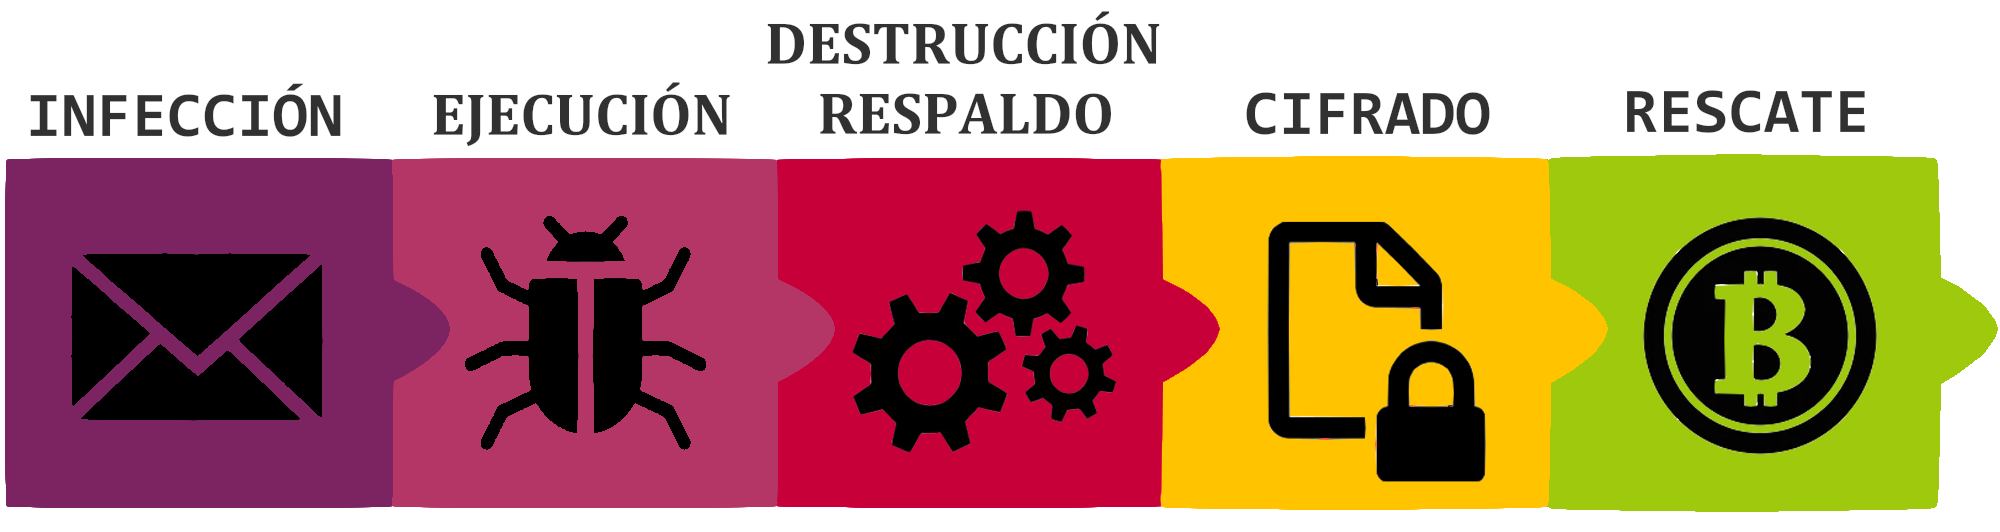
\includegraphics{images/etapas-ataque.png}}}
\end{center}
\caption{Patrón de ataque de un ransomware.}
\label{fig:imstages}
\end{figure}



\subsection{Métodos de Cifrado}
\noindent El ransomware moderno, como WannaCry, Petya o Locky, utiliza esquemas de cifrado híbrido, dificultando aún más la labor de recuperar la información cifrada en el ataque \cite{ransEncr}. A continuación se exponen los métodos de cifrado de archivos más importantes \cite{cypher}:

\begin{enumerate}
    \item \textbf{Cifrado simétrico}: También denominado cifrado de clave secreta. El texto plano se cifra y se descifra con la misma clave. La seguridad del cifrado no depende del algoritmo, si no de la privacidad de la clave. Permite que el ransomware cifre los datos a gran velocidad, y posteriormente almacena en disco las claves para almacenar cada archivo. Existen dos tipos de algoritmos simétricos:
    \begin{itemize}
        \item \textbf{Cifrado de bloque}: Procesa la entrada del texto en bloques de tamaño fijo y produce un texto cifrado de igual tamaño. Los más importantes son \gls{DES}, \gls{3DES}, vistos en la Figura \ref{fig:imdes} y \gls{AES}.
        
        \begin{figure}[htb!]
        \begin{center}
        \subfigure[Cifrado]{
            {\scalebox{.93}{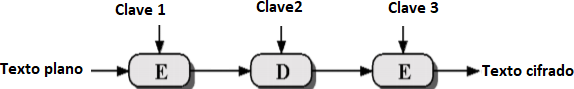
\includegraphics{images/3des_1.png}}}
            \label{fig:des1}}
        \subfigure[Descifrado]{
            {\scalebox{.93}{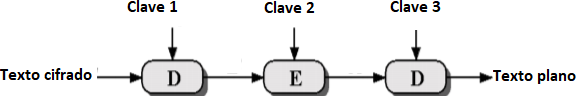
\includegraphics{images/3des_2.png}}}
            \label{fig:des2}}
        \caption{El algoritmo 3DES aplica 3 veces el algoritmo DES con claves distintas}
        \label{fig:imdes}
        \end{center}
        \end{figure}
        
        \item \textbf{Cifrado de flujo}: Procesa elementos de entrada y produce un elemento de salida. El más importante es \gls{RC4}.
        
    \end{itemize}
    
    \item \textbf{Cifrado asimétrico}: También denominado cifrado de clave pública. Está basado en funciones matemáticas en lugar de usar operaciones binarias sobre patrones de bits, por lo tanto este cifrado es más lento. Usa dos claves distintas: una pública y otra privada. El ransomware utiliza la clave pública para cifrar los archivos, y la clave privada es enviada al servidor de mando y control para ser almacenada, por lo que se necesita una conexión a internet. Los algoritmos más utilizados son \gls{DSA}, \gls{RSA} y \gls{DH}. Se diferencian las siguientes aplicaciones:
    \begin{itemize}
        \item \textbf{Cifrado con clave pública}: El emisor cifra con la clave pública del receptor y el receptor descifra con la clave privada.
        \item \textbf{Intercambio de clave}: Dos partes cooperan para establecer una clave secreta compartida.
        \item \textbf{Firma digital}: técnica utilizada para asegurar la autenticación y la integridad de los datos.
        \item \textbf{Certificado digital}: Se utiliza para proporcionar autenticación de las partes y no repudio
    \end{itemize}
    
    \item \textbf{Cifrado híbrido}: Usa cifrado simétrico y asimétrico. No necesita conexión a internet en el cifrado, pero sí en el descifrado. El ransomware y el servidor de mando y control generan un par de claves. Se cifrará la clave privada del cliente utilizando la clave pública del servidor. Al finalizar, todas las claves serán cifradas con la clave pública del cliente. Un ejemplo es el algoritmo utilizado por Locky: \gls{RSA}-2048+\gls{AES}-128 \cite{ransEncr}.
\end{enumerate}

\section{Detección}\label{sec:2-8}
\noindent Las técnicas usadas por los software de antivirus para reconocer la presencia de ransomware en el equipo son las siguientes \cite{ransommasive}:
\begin{itemize}
    \item \textbf{Detección basada en firma digital}: Cuando la compañía del antivirus descubre el malware crea una firma única para el tipo en concreto, y actualiza la base de datos del antivirus para poder comparar y capturar cuando el malware intente acceder a dicho equipo. No puede detectar avanzados tipos de malware polimórficos o que utilizan técnicas de cifrado para evadir dicha detección. 
    \item \textbf{Análisis del comportamiento}: Esta técnica trata de identificar el malware mediante los cambios que produce en el sistema, como puede ser la eliminación de ficheros, el aumento de la entropía (para cifrar los ficheros), las conexiones a redes extrañas, etc. Para recopilar estos datos, una técnica es registrar las llamadas a las \gls{API}s, los recursos del sistema que se están utilizando, los archivos que abre cada proceso, e introducirlas en una solución de \gls{ML} que sea capaz de detectar si esa serie de llamadas pueda corresponder a la ejecución de un ransomware \cite{Arabo2020}. 
    \item \textbf{Detección heurística}: Se basa en reglas y algoritmos para analizar si el código es malicioso. Puede realizarse un análisis estático, mediante un estudio de los indicadores sin ejecución como anomalías estructurales del código, el desmontaje del programa o el estudio de los elementos de una secuencia dada (n-gramas). Análogamente, el análisis dinámico, realiza un estudio de los indicadores del código en ejecución mediante técnicas de \textit{sandboxing} o virtualización \cite{DUBE2012137}. 
    \item \textbf{Detección usando la nube}: El archivo sospechoso se envía a un antivirus en la infraestructura de la nube del vendedor, aprovechando la capacidad computacional de la plataforma para analizarla de manera más rápida y eficiente. 
\end{itemize}

Además de las técnicas usadas por los antivirus y debido a que un ransomware puede cifrar archivos en cuestión de minutos, es importante implementar una detección a tiempo real tanto en el ordenador del usuario como en servidores web. Para implementar esta detección es importante seguir estos pasos \cite{74}:
\begin{itemize}
\item \textbf{Implementar escáneres de vulnerabilidad}: Se necesita saber en todo momento la información del sistema y de sus archivos tanto en local como en la nube. 
\item \textbf{Detección de intrusiones}: El ransomware es difícil de detectar antes de que ataque, pero un buen sistema de detección de intrusiones puede ser lo suficientemente rápido como para frenarlo antes de que cifre algún archivo. Un sistema de detección de intrusiones puede detectar comportamientos característicos de un ataque de ransomware en sus etapas iniciales \cite{107}. Algunos ejemplos de estos comportamientos son: deshabilitar el cortafuegos o el software antivirus, iniciar escáneres de red no autorizados, enviar datos a través de un canal encubierto y actualizar la política de auditoría.
\item \textbf{Activar la monitorización de la integridad de archivos}: Una parte principal del malware, incluyendo el ransomware, es ejecutar procesos para obtener permisos que le permitan acceder a los archivos del sistema. Estos procesos no se ejecutan normalmente, por lo que la monitorización de la integridad de los archivos puede generar una alerta cada vez que los detecta. Esto no va a prevenir el inicio del cifrado de archivos, pero puede evitar futuros ataques y poder aislar y poner en cuarentena el sistema infectado \cite{108}.
\item \textbf{Implementar la automatización de la seguridad}: Una respuesta rápida es un factor crítico de éxito en cualquier tipo de emergencia. Las innovaciones en el sector de la automatización y gestión de la seguridad han mejorado significativamente la respuesta ante amenazas, asegurando el funcionamiento conjunto de varias herramientas de seguridad. Este enfoque puede proporcionar una desconexión inmediata de la red y el aislamiento de los sistemas cuando se detecten las actividades del ransomware \cite{109}.
\item \textbf{Gestionar y analizar los registros}: Los objetivos del atacante se encuentran en los registros del sistema, de las aplicaciones, de la actividad... Detectar el acceso a los registros es complicado debido a la gran cantidad de ellos, por lo que es necesario automatizar su gestión y análisis.
\item \textbf{Combinar inteligencia sobre amenazas con la monitorización del sistema}: Los desarrolladores de ransomware más experimentados están en constantemente evolucionando sus métodos y código. Los analistas de seguridad deben investigan cuidadosamente su desarrollo, innovación e infraestructura para desarrollar métodos de gestión pro-activos (por ejemplo, software para la correlación de eventos) y herramientas para detectar los últimos ataques de ransomware.
\end{itemize}

\section{Prevención}\label{sec:2-9}

\noindent Se diferencian las estrategias de defensa que siguen las empresas contra los ataques ransomware y las acciones que han de seguir los usuarios finales para no estar expuestos \cite{ransommasive}.

\subsection{Defensa Individualizada}
\noindent La seguridad del equipo del usuario final es clave para proteger la red entera de una organización, puesto que basta con infectar un equipo para que algunos tipos de ransomware puedan propagarse por la totalidad de ellos. Al contrario de lo que piensa mucha gente, no basta solo con instalar un antivirus, sino que hay que cumplir una serie de acciones para alcanzar un grado de seguridad superior \cite{ransommasive}:
\begin{itemize}
    \item \textbf{Mantener respaldo de los datos}: Si los datos cifrados estaban replicados de manera consistente en otro dispositivo o en la nube, se pueden recuperar sin problema sin tener que pagar ningún rescate.
    
    \item \textbf{Mantener el sistema operativo y las aplicaciones actualizadas}: Sirven para arreglar las vulnerabilidades detectadas. El sistema operativo debe estar configurado para actualizarse tan pronto como la actualización esté disponible. Esto permitirá que el sistema sea más seguro frente a las vulnerabilidades, los kits de \textit{exploit}, etc. 
    
    \item \textbf{Uso de la virtualización}: El uso de máquinas virtuales permite ejecutar programas, descargarlos de internet y visitar páginas web comprometidas debido a que se ejecuta en un entorno seguro aislado del sistema operativo raíz. Aun así se debe mantener la precaución de que no el ransomware no se propague por la red en la que se encontraba la máquina virtual.
    
    \item \textbf{Bloquear la redirección web}: Esto evita páginas web no deseadas y enlaces maliciosos. Los navegadores actuales permiten esta configuración. También es buena práctica añadir extensiones al navegador para bloquear anuncios y \textit{pop ups} maliciosos, incluso algunas como \href{https://noscript.net/}{\textcolor{blue}{NoScript}}, que únicamente permite que se ejecuten los \textit{plugins} en los sitios web establecidos por el usuario.
    
    \item \textbf{Deshabilitar macros de Microsoft Office}: Como se ha explicado en la Sección \ref{item:macros} esta característica puede ser explotada para introducir ransomware en el equipo víctima. Además, es aconsejable abrir los archivos de Office recibidos vía correo electrónico en otra plataforma como Google Docs.
    
    \item \textbf{Dipositivos \gls{USB}}: Está totalmente desaconsejado conectar dispositivos desconocidos, poco fiables o encontrados en el sistema, puesto que puede contener ransomware que se instale al conectarlo. En algún caso, se debe configurar el antivirus para que escanee la unidad antes de montarla.
    
    \item \textbf{Modificar la extensión de los archivos importantes}: Algunos tipos de ransomware como WannaCry, cifran los ficheros basándose en una búsqueda por la extensión.
    
    \item \textbf{Remote Desktop Protocol}: Este protocolo permite el acceso remoto a un ordenador, de manera que si un atacante se conecta, podría infectar el equipo. Para restringir el acceso se recomienda utilizar una contraseña consistente, utilizar sesiones \gls{VPN} fiables y asegurarse de permitir conexiones autenticadas a nivel de red (\gls{NLA}).
\end{itemize}

\subsection{Estrategias Empresariales}
\noindent De manera complementaria a las medidas de seguridad que deben tomar los usuarios finales vistas en el apartado anterior, las organizaciones, empresas y gobiernos siguen una serie de estrategias de prevención en contra del auge de los ataques ransomware \cite{ransommasive}. 

\begin{itemize}
    \item \textbf{Seguridad física}: La seguridad de los equipos digitales (servidores, almacenamiento del respaldo, ordenadores, dispositivos de red) es tan importante como la de los datos almacenados en ellos. Para asegurarlos, se deben cumplir una serie de reglas como la restricción del acceso con medidas biométricas, monitorizar y restringir los espacios, no dejar equipos desatendidos, desconectar de la red sistemas sin utilizar, etc. 
    \item \textbf{Segmentación de red}: Es una medida para luchar contra el ransomware que limita la posibilidad del atacante de acceder al segmento donde se encuentra la información sensible. En la Figura \ref{fig:im11} de pueden ver las ventajas de esta segmentación.
    \begin{figure}[htb]
    \begin{center}
    {\scalebox{.9}{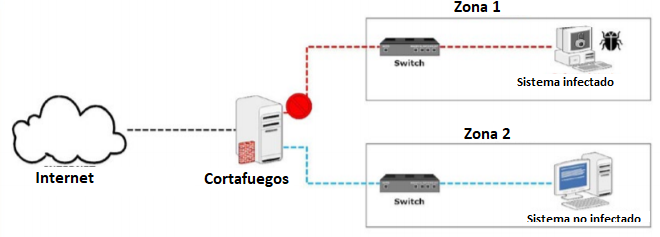
\includegraphics{images/segmentacion.png}}}
    \end{center}
    \caption{Ventajas de la segmentación de la red}
    \label{fig:im11}
    \end{figure}
    \item \textbf{Cortafuegos modernos}: Cualquier plan de seguridad comienza instalando un cortafuegos en el perímetro de la red, limitando las conexiones y permitiendo solo las permitidas. Los de nueva generación añaden otras herramientas de seguridad como antivirus, antimalware y el soporte para las redes privadas virtuales (\gls{VPN}).
    \item \textbf{Seguridad de correo electrónico}: Puesto que es el acceso más utilizado por el ransomware se deben desarrollar sistemas de filtrado avanzado de \textit{spam} mediante filtrado de \gls{IP} y contenido y deshabilitar el código \gls{HTML} en los e-mails recibidos por texto plano.
    \item \textbf{Formación de los trabajadores}: Para la creación de un entorno seguro, los trabajadores de la organización deben ser conscientes del riesgo existente y poner a su disposición la formación necesaria y los hábitos que deben seguir, como utilizar contraseñas seguras, no acceder a enlaces ni descargas de e-mails desconocidos, no conectar dispositivos extraños, etc \cite{TOPAYORNOT}.
    \item \textbf{Honeypots}: Se tratan de señuelos con información falsa que se anuncian online como objetivos de valor para cibercriminales y que permiten la detección de los ataques. En la Figura \ref{fig:im10} se aprecia el funcionamiento de honeypot.
    \begin{figure}[htb]
        \begin{center}
        {\scalebox{.9}{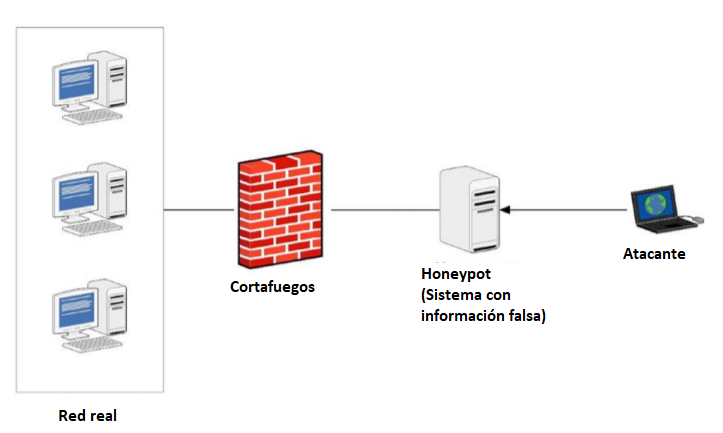
\includegraphics{images/honeypot.png}}}
        \end{center}
        \caption{Funcionamiento de honeypot}
        \label{fig:im10}
    \end{figure}
\end{itemize}


\section{Período Post-ataque}\label{sec:2-10}
\noindent Una vez el sistema ha sido infectado, se plantea una cuestión fundamental: ¿se debe pagar el rescate para recuperar el equipo infectado? La respuesta de los expertos es clara: no. Por un lado, te convertirías en un mayor objetivo, puesto que esta información es compartida entre atacantes, y conociendo que ya has pagado una vez, podrás hacerlo en otras ocasiones. Además, aunque cada vez más los criminales están cumpliendo con devolver los archivos (un ejemplo de ello es Cryptolocker, que permite descifrar 5 archivos elegidos de manera gratuita) debido a que creando esta confianza, más gente pagará por el rescate,  no se puede establecer confianza en los cibercriminales y en que el equipo sea descifrado. Por último, pagar el rescate provoca que los cibercriminales tengan más motivos para seguir con su labor \cite{TOPAYORNOT}. 

Si se ha decidido no pagar el rescate por los datos cifrados todavía se puede albergar alguna esperanza. Se debe realizar una valoración para conocer si se pueden recuperar los archivos cifrados siguiendo unos pasos \cite{CcnCert}:
\begin{enumerate}
    \item \textbf{Respaldo}: Si se dispone de una copia de seguridad, se procede a la desinfección del sistema y a la restauración de la copia de seguridad.
    \item \textbf{Herramientas de descifrado}: Aunque existen pocas variantes de ransomware que se puedan descifrar, por la intervención del \gls{CyC} y se han obtenido las claves, o porque existen vulnerabilidades en el código malicioso, hay disponibles herramientas públicas para descifrar archivos atacados por ransomware concreto, que se listan en la Tabla \ref{tab:recu}.
    

    \item \textbf{Shadow Volume Copy}: Si el ransomware no ha deshabilitado esta función como se ha expuesto previamente, se podrían restaurar los datos que Windows duplica automáticamente estableciendo una copia de seguridad.
    \item \textbf{Software forense}: En algunos casos es factible la recuperación de algunos ficheros originales mediante programas de análisis forense.
\end{enumerate}



    \begin{table}[htb!]
    \centering
    \scriptsize %para hacer la tabla mas pequeña
    \caption{Herramientas para la recuperación de datos}
    \begin{tabular}{|c|p{11.9cm}|}
        \hline
        \rowcolor[HTML]{C0C0C0}
        \textbf{Ransomware} &
        \multicolumn{1}{c|}{\cellcolor[HTML]{C0C0C0}{\textbf{Recuperación de ficheros}}} \\ \hline
        \textbf{Cerber}  &   En las versiones 1 y 2 herramienta Check Point. Versiones posteriores mediante 
        copia de seguridad \\ \hline
        \textbf{Crytolocker} & Comprobar en la web \url{http://www.decryptcryptolocker.com/} por si existe solución para su caso \\ \hline
        \textbf{Locky} & Comprobar mediante la herramienta Autolocky \\ \hline
        \textbf{Petya} & Primera versión: herramienta Bleepingcomputer. Segunda versión: publicada la clave privada. \\ \hline
        \textbf{Wannacry} & Solo mediante copia de seguridad. \\ \hline
        \textbf{Crysis}  & Algunas variantes mediante RakhniDecryptor \\ \hline
        \textbf{NotPetya}    & Solo mediante copia de seguridad \\ \hline
        \textbf{Cryptowall}  & Tercera versión mediante herramientas de recuperación de ficheros. Las demás versiones mediante copia de seguridad. \\ \hline
        \textbf{Cryptodefense} & Herramienta Emsisoft. \\ \hline 
    \end{tabular}
    \label{tab:recu}
    \end{table}